\documentclass[ twoside,openright,titlepage,numbers=noenddot,headinclude,%1headlines,% letterpaper a4paper
                footinclude=true,cleardoublepage=empty,abstractoff, % <--- obsolete, remove (todo)
                BCOR=5mm,paper=a4,fontsize=11pt,%11pt,a4paper,%
                ngerman,american,%
                ]{scrreprt}


%load fonts und useful packages. etc.
\input{config}
\begin{document}
\frenchspacing
\raggedbottom
\selectlanguage{american} % american ngerman
%\renewcommand*{\bibname}{new name}
%\setbibpreamble{}
\pagenumbering{roman}
\pagestyle{plain}
%create titelpage
\include{FrontBackmatter/Titlepage}
%\include{FrontBackmatter/Contents}
\pagestyle{scrheadings}


\pagenumbering{arabic}

\chapter{Motivation and Implementation}
\section{Introduction}
In this project we are going to find the optimal path for a solar powered airplane \footnote{Like the one from \url{http://www.solarimpulse.com/}}. During flight the plane's electrical engines drain power from it's battery, while at the same time solar panels on the plane's wings convert energy from the sun's rays into electric energy. However clouds may block the sun's rays from reaching the panels. In addition the suns intensity increases when flying closer to the earth's equator. In order to keep as much energy in the planes batteries as possible the flight path has to be optimized.

\section{Problem formulation and Analysis}
In the optimization process we use randomly generated weather data and sun data corresponding to a flight between $48^\circ$ and $50^\circ$ latitude. We generate the weather data by cubicly interpolating a random matrix of size \texttt{n} over a grid. The larger n becomes the more complex the weather will be. This functionality is implemented in \texttt{Static\_Weather.m} \footnote{All matlab code can be found on \url{https://github.com/double2double/OptimisationProject/} in the MATLAB folder.} The class returns a weather data matrix $W$.
Data for the sun comes from a couple of established equations that relate the local time and position to the sun's intensity  which happens in \texttt{sun.m}. The class returns a sun data Matrix $S$. We define low values in the weather Data Matrix as cloudy and high values as sunny weather. As clouds reduce the electric yield of our plane's solar cells we define the overall intensity as:
\begin{equation}
$I$ \:= \: $W$ .* $S$
\end{equation}
While following a convention where $.*$ denotes element wise multiplication we end up with an intensity matrix $I$, which contains sun intensity data weighted according to the random weather.

Next we took a closer look at the airplane. Here we consider the degree to which the plane can recharge its battery during flight, which is the path integral over the intensity data:
\begin{equation}
\oint_{path}
\end{equation} 


\section{Optimisation Algorithm description}

\chapter{Results}
\begin{figure}
% This file was created by matlab2tikz v0.4.7 running on MATLAB 8.4.
% Copyright (c) 2008--2014, Nico Schlömer <nico.schloemer@gmail.com>
% All rights reserved.
% Minimal pgfplots version: 1.3
% 
% The latest updates can be retrieved from
%   http://www.mathworks.com/matlabcentral/fileexchange/22022-matlab2tikz
% where you can also make suggestions and rate matlab2tikz.
% 
\documentclass[tikz]{standalone}
\usepackage{pgfplots}
\usepackage{grffile}
\pgfplotsset{compat=newest}
\usetikzlibrary{plotmarks}
\usepackage{amsmath}

\begin{document}
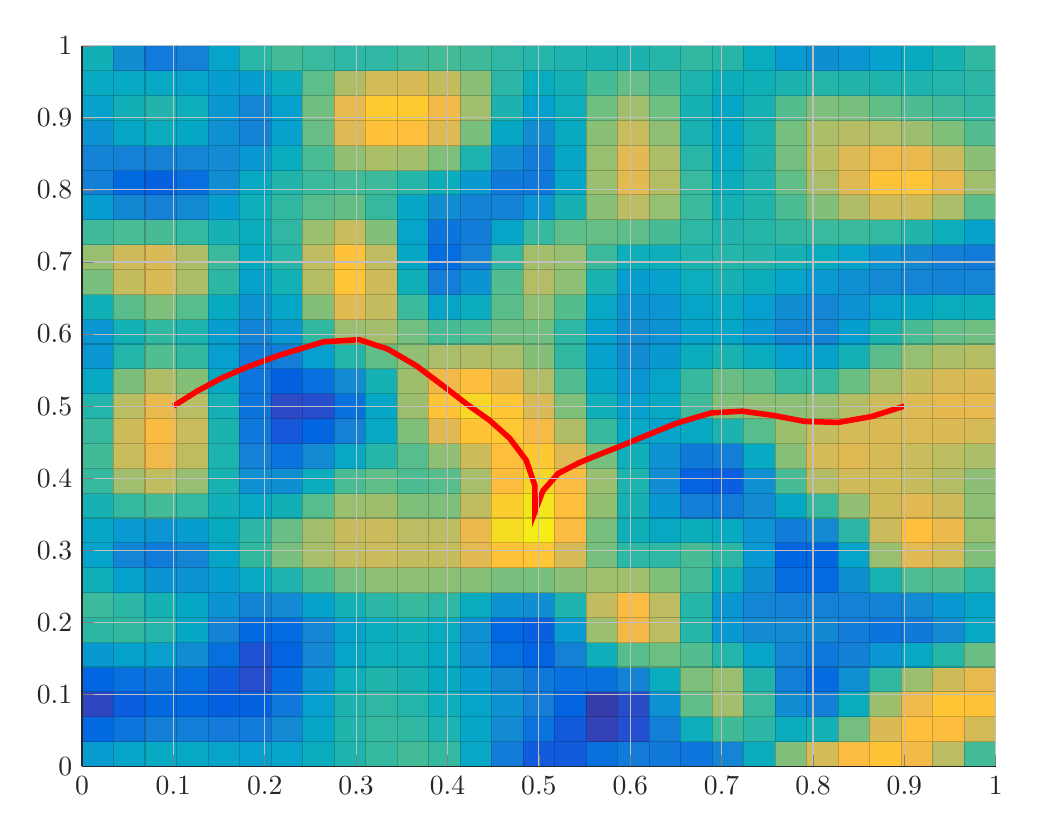
\begin{tikzpicture}

\begin{axis}[%
width=4.56842105263158in,
height=3.60315789473684in,
view={0}{90},
scale only axis,
every outer x axis line/.append style={white!15!black},
every x tick label/.append style={font=\color{white!15!black}},
xmin=0,
xmax=1,
xmajorgrids,
every outer y axis line/.append style={white!15!black},
every y tick label/.append style={font=\color{white!15!black}},
ymin=0,
ymax=1,
ymajorgrids,
every outer z axis line/.append style={white!15!black},
every z tick label/.append style={font=\color{white!15!black}},
zmin=-0.00225506975800025,
zmax=3,
ztick={\empty},
zmajorgrids,
axis x line*=bottom,
axis y line*=left,
axis z line*=left
]

\addplot3[%
surf,
shader=faceted,
draw=black,
colormap={mymap}{[1pt] rgb(0pt)=(0.2081,0.1663,0.5292); rgb(1pt)=(0.211624,0.189781,0.577676); rgb(2pt)=(0.212252,0.213771,0.626971); rgb(3pt)=(0.2081,0.2386,0.677086); rgb(4pt)=(0.195905,0.264457,0.7279); rgb(5pt)=(0.170729,0.291938,0.779248); rgb(6pt)=(0.125271,0.324243,0.830271); rgb(7pt)=(0.0591333,0.359833,0.868333); rgb(8pt)=(0.0116952,0.38751,0.881957); rgb(9pt)=(0.00595714,0.408614,0.882843); rgb(10pt)=(0.0165143,0.4266,0.878633); rgb(11pt)=(0.0328524,0.443043,0.871957); rgb(12pt)=(0.0498143,0.458571,0.864057); rgb(13pt)=(0.0629333,0.47369,0.855438); rgb(14pt)=(0.0722667,0.488667,0.8467); rgb(15pt)=(0.0779429,0.503986,0.838371); rgb(16pt)=(0.0793476,0.520024,0.831181); rgb(17pt)=(0.0749429,0.537543,0.826271); rgb(18pt)=(0.0640571,0.556986,0.823957); rgb(19pt)=(0.0487714,0.577224,0.822829); rgb(20pt)=(0.0343429,0.596581,0.819852); rgb(21pt)=(0.0265,0.6137,0.8135); rgb(22pt)=(0.0238905,0.628662,0.803762); rgb(23pt)=(0.0230905,0.641786,0.791267); rgb(24pt)=(0.0227714,0.653486,0.776757); rgb(25pt)=(0.0266619,0.664195,0.760719); rgb(26pt)=(0.0383714,0.674271,0.743552); rgb(27pt)=(0.0589714,0.683757,0.725386); rgb(28pt)=(0.0843,0.692833,0.706167); rgb(29pt)=(0.113295,0.7015,0.685857); rgb(30pt)=(0.145271,0.709757,0.664629); rgb(31pt)=(0.180133,0.717657,0.642433); rgb(32pt)=(0.217829,0.725043,0.619262); rgb(33pt)=(0.258643,0.731714,0.595429); rgb(34pt)=(0.302171,0.737605,0.571186); rgb(35pt)=(0.348167,0.742433,0.547267); rgb(36pt)=(0.395257,0.7459,0.524443); rgb(37pt)=(0.44201,0.748081,0.503314); rgb(38pt)=(0.487124,0.749062,0.483976); rgb(39pt)=(0.530029,0.749114,0.466114); rgb(40pt)=(0.570857,0.748519,0.44939); rgb(41pt)=(0.609852,0.747314,0.433686); rgb(42pt)=(0.6473,0.7456,0.4188); rgb(43pt)=(0.683419,0.743476,0.404433); rgb(44pt)=(0.71841,0.741133,0.390476); rgb(45pt)=(0.752486,0.7384,0.376814); rgb(46pt)=(0.785843,0.735567,0.363271); rgb(47pt)=(0.818505,0.732733,0.34979); rgb(48pt)=(0.850657,0.7299,0.336029); rgb(49pt)=(0.882433,0.727433,0.3217); rgb(50pt)=(0.913933,0.725786,0.306276); rgb(51pt)=(0.944957,0.726114,0.288643); rgb(52pt)=(0.973895,0.731395,0.266648); rgb(53pt)=(0.993771,0.745457,0.240348); rgb(54pt)=(0.999043,0.765314,0.216414); rgb(55pt)=(0.995533,0.786057,0.196652); rgb(56pt)=(0.988,0.8066,0.179367); rgb(57pt)=(0.978857,0.827143,0.163314); rgb(58pt)=(0.9697,0.848138,0.147452); rgb(59pt)=(0.962586,0.870514,0.1309); rgb(60pt)=(0.958871,0.8949,0.113243); rgb(61pt)=(0.959824,0.921833,0.0948381); rgb(62pt)=(0.9661,0.951443,0.0755333); rgb(63pt)=(0.9763,0.9831,0.0538)},
mesh/rows=30]
table[row sep=crcr,header=false] {0	0	0.118352773742808\\
0	0.0344827586206897	0.051402733664511\\
0	0.0689655172413793	0.0144955025456188\\
0	0.103448275862069	0.00799732940231117\\
0	0.137931034482759	0.0504457738476799\\
0	0.172413793103448	0.116305609098239\\
0	0.206896551724138	0.153409403343879\\
0	0.241379310344828	0.148710065697585\\
0	0.275862068965517	0.128988519473172\\
0	0.310344827586207	0.11814035138516\\
0	0.344827586206897	0.117198106800518\\
0	0.379310344827586	0.117538221760774\\
0	0.413793103448276	0.113677736703432\\
0	0.448275862068965	0.106044979487242\\
0	0.482758620689655	0.0965034881059803\\
0	0.517241379310345	0.0842361113476219\\
0	0.551724137931034	0.0645078897232184\\
0	0.586206896551724	0.0540427263920414\\
0	0.620689655172414	0.0744611779370698\\
0	0.655172413793103	0.126309556134795\\
0	0.689655172413793	0.168526183532657\\
0	0.724137931034483	0.16386110191874\\
0	0.758620689655172	0.125380066955824\\
0	0.793103448275862	0.0881364029872505\\
0	0.827586206896552	0.072677828640544\\
0	0.862068965517241	0.0668806979302004\\
0	0.896551724137931	0.0735481583751604\\
0	0.931034482758621	0.0944243086902338\\
0	0.96551724137931	0.128353456496835\\
0	1	0.175373514681729\\
0.0344827586206897	0	0.133051801904348\\
0.0344827586206897	0.0344827586206897	0.0669327133402057\\
0.0344827586206897	0.0689655172413793	0.0299940420564649\\
0.0344827586206897	0.103448275862069	0.0226197381365943\\
0.0344827586206897	0.137931034482759	0.0649266931826866\\
0.0344827586206897	0.172413793103448	0.129171179621575\\
0.0344827586206897	0.206896551724138	0.15827702502747\\
0.0344827586206897	0.241379310344828	0.12996101475779\\
0.0344827586206897	0.275862068965517	0.0871250092903166\\
0.0344827586206897	0.310344827586207	0.078702434972271\\
0.0344827586206897	0.344827586206897	0.114766846146786\\
0.0344827586206897	0.379310344827586	0.161304075995182\\
0.0344827586206897	0.413793103448276	0.185590452852345\\
0.0344827586206897	0.448275862068965	0.191750945245977\\
0.0344827586206897	0.482758620689655	0.186881925234792\\
0.0344827586206897	0.517241379310345	0.169995891204855\\
0.0344827586206897	0.551724137931034	0.132825062589305\\
0.0344827586206897	0.586206896551724	0.103969816338456\\
0.0344827586206897	0.620689655172414	0.118344416082904\\
0.0344827586206897	0.655172413793103	0.174665736004839\\
0.0344827586206897	0.689655172413793	0.216615116701535\\
0.0344827586206897	0.724137931034483	0.19027258156996\\
0.0344827586206897	0.758620689655172	0.112683455229781\\
0.0344827586206897	0.793103448275862	0.048776491137308\\
0.0344827586206897	0.827586206896552	0.0482088331629678\\
0.0344827586206897	0.862068965517241	0.0844715020053526\\
0.0344827586206897	0.896551724137931	0.11440568612681\\
0.0344827586206897	0.931034482758621	0.11701169982441\\
0.0344827586206897	0.96551724137931	0.107227310550705\\
0.0344827586206897	1	0.0852026183574342\\
0.0689655172413793	0	0.141486259314942\\
0.0689655172413793	0.0344827586206897	0.0776366884727265\\
0.0689655172413793	0.0689655172413793	0.0411418631588219\\
0.0689655172413793	0.103448275862069	0.0323722564806591\\
0.0689655172413793	0.137931034482759	0.0709744704071807\\
0.0689655172413793	0.172413793103448	0.129842372396177\\
0.0689655172413793	0.206896551724138	0.153020910253856\\
0.0689655172413793	0.241379310344828	0.114888844405272\\
0.0689655172413793	0.275862068965517	0.0639232654085365\\
0.0689655172413793	0.310344827586207	0.0588951673358285\\
0.0689655172413793	0.344827586206897	0.114304808497332\\
0.0689655172413793	0.379310344827586	0.18436111222759\\
0.0689655172413793	0.413793103448276	0.223262493395279\\
0.0689655172413793	0.448275862068965	0.236904595522593\\
0.0689655172413793	0.482758620689655	0.234902405485745\\
0.0689655172413793	0.517241379310345	0.216242494816764\\
0.0689655172413793	0.551724137931034	0.171067397348964\\
0.0689655172413793	0.586206896551724	0.133260409146075\\
0.0689655172413793	0.620689655172414	0.143532933042141\\
0.0689655172413793	0.655172413793103	0.199658337989242\\
0.0689655172413793	0.689655172413793	0.239334413613678\\
0.0689655172413793	0.724137931034483	0.20170280206649\\
0.0689655172413793	0.758620689655172	0.105252723452515\\
0.0689655172413793	0.793103448275862	0.0289588217363666\\
0.0689655172413793	0.827586206896552	0.0368264919521401\\
0.0689655172413793	0.862068965517241	0.0953515536560926\\
0.0689655172413793	0.896551724137931	0.137009845160383\\
0.0689655172413793	0.931034482758621	0.128727331132009\\
0.0689655172413793	0.96551724137931	0.0939815259081873\\
0.0689655172413793	1	0.032979695607701\\
0.103448275862069	0	0.143597838796122\\
0.103448275862069	0.0344827586206897	0.0834467888783432\\
0.103448275862069	0.0689655172413793	0.0478580079475322\\
0.103448275862069	0.103448275862069	0.0371570633400334\\
0.103448275862069	0.137931034482759	0.0684530485320537\\
0.103448275862069	0.172413793103448	0.118147996227669\\
0.103448275862069	0.206896551724138	0.137489871683163\\
0.103448275862069	0.241379310344828	0.103471953548799\\
0.103448275862069	0.275862068965517	0.0595039009241212\\
0.103448275862069	0.310344827586207	0.0588527872721051\\
0.103448275862069	0.344827586206897	0.115787348529833\\
0.103448275862069	0.379310344827586	0.18648189324557\\
0.103448275862069	0.413793103448276	0.226355627255373\\
0.103448275862069	0.448275862068965	0.241137143937756\\
0.103448275862069	0.482758620689655	0.240202449717333\\
0.103448275862069	0.517241379310345	0.222636246098268\\
0.103448275862069	0.551724137931034	0.178952292860701\\
0.103448275862069	0.586206896551724	0.141684248807479\\
0.103448275862069	0.620689655172414	0.149792004190184\\
0.103448275862069	0.655172413793103	0.200991870386644\\
0.103448275862069	0.689655172413793	0.236362281291979\\
0.103448275862069	0.724137931034483	0.197938578164012\\
0.103448275862069	0.758620689655172	0.103093616389193\\
0.103448275862069	0.793103448275862	0.0288435117516358\\
0.103448275862069	0.827586206896552	0.0386179472720639\\
0.103448275862069	0.862068965517241	0.0993892475661005\\
0.103448275862069	0.896551724137931	0.141100612127285\\
0.103448275862069	0.931034482758621	0.129389752354533\\
0.103448275862069	0.96551724137931	0.0886376721766004\\
0.103448275862069	1	0.0190532064299762\\
0.137931034482759	0	0.135299639717406\\
0.137931034482759	0.0344827586206897	0.0795022777920944\\
0.137931034482759	0.0689655172413793	0.044283279563702\\
0.137931034482759	0.103448275862069	0.0298745753981053\\
0.137931034482759	0.137931034482759	0.0475514112902892\\
0.137931034482759	0.172413793103448	0.0818047108644439\\
0.137931034482759	0.206896551724138	0.100802849782935\\
0.137931034482759	0.241379310344828	0.0939216749227482\\
0.137931034482759	0.275862068965517	0.0820647164882248\\
0.137931034482759	0.310344827586207	0.0877531598607738\\
0.137931034482759	0.344827586206897	0.11728571045659\\
0.137931034482759	0.379310344827586	0.151568743274301\\
0.137931034482759	0.413793103448276	0.171083872234316\\
0.137931034482759	0.448275862068965	0.178658786914007\\
0.137931034482759	0.482758620689655	0.17754707317075\\
0.137931034482759	0.517241379310345	0.165525211592339\\
0.137931034482759	0.551724137931034	0.136682274411662\\
0.137931034482759	0.586206896551724	0.11294257356728\\
0.137931034482759	0.620689655172414	0.12040120321285\\
0.137931034482759	0.655172413793103	0.157604105553331\\
0.137931034482759	0.689655172413793	0.184755257128543\\
0.137931034482759	0.724137931034483	0.16369761558911\\
0.137931034482759	0.758620689655172	0.106398430074816\\
0.137931034482759	0.793103448275862	0.059533717062264\\
0.137931034482759	0.827586206896552	0.059517665505532\\
0.137931034482759	0.862068965517241	0.0870452414074104\\
0.137931034482759	0.896551724137931	0.108051058217735\\
0.137931034482759	0.931034482758621	0.105915246617677\\
0.137931034482759	0.96551724137931	0.0924492499579433\\
0.137931034482759	1	0.0677654529819487\\
0.172413793103448	0	0.122285010826383\\
0.172413793103448	0.0344827586206897	0.0725778595994218\\
0.172413793103448	0.0689655172413793	0.0385859336747086\\
0.172413793103448	0.103448275862069	0.0204228897614719\\
0.172413793103448	0.137931034482759	0.0219459050668695\\
0.172413793103448	0.172413793103448	0.0379333147093765\\
0.172413793103448	0.206896551724138	0.0581271638401765\\
0.172413793103448	0.241379310344828	0.0887386657290751\\
0.172413793103448	0.275862068965517	0.120193907782249\\
0.172413793103448	0.310344827586207	0.132818366787452\\
0.172413793103448	0.344827586206897	0.121493303632934\\
0.172413793103448	0.379310344827586	0.102051892496468\\
0.172413793103448	0.413793103448276	0.0905852818114294\\
0.172413793103448	0.448275862068965	0.0853945618560068\\
0.172413793103448	0.482758620689655	0.0820847498025457\\
0.172413793103448	0.517241379310345	0.0778530505902464\\
0.172413793103448	0.551724137931034	0.0718361994951512\\
0.172413793103448	0.586206896551724	0.06974580612522\\
0.172413793103448	0.620689655172414	0.0786618708391407\\
0.172413793103448	0.655172413793103	0.0988474776934657\\
0.172413793103448	0.689655172413793	0.116487682454615\\
0.172413793103448	0.724137931034483	0.120280163677554\\
0.172413793103448	0.758620689655172	0.114906102016436\\
0.172413793103448	0.793103448275862	0.105565901196989\\
0.172413793103448	0.827586206896552	0.0912641690783366\\
0.172413793103448	0.862068965517241	0.0716186414684238\\
0.172413793103448	0.896551724137931	0.0638226755044452\\
0.172413793103448	0.931034482758621	0.0765420986199597\\
0.172413793103448	0.96551724137931	0.103678432988704\\
0.172413793103448	1	0.145208765661568\\
0.206896551724138	0	0.116090220303241\\
0.206896551724138	0.0344827586206897	0.0766127372223685\\
0.206896551724138	0.0689655172413793	0.0476740654333492\\
0.206896551724138	0.103448275862069	0.0292931682516207\\
0.206896551724138	0.137931034482759	0.0197683366499497\\
0.206896551724138	0.172413793103448	0.0215721727258632\\
0.206896551724138	0.206896551724138	0.0404833361177542\\
0.206896551724138	0.241379310344828	0.0932245451357916\\
0.206896551724138	0.275862068965517	0.150961116888334\\
0.206896551724138	0.310344827586207	0.168359129949028\\
0.206896551724138	0.344827586206897	0.134183100038607\\
0.206896551724138	0.379310344827586	0.083792824115459\\
0.206896551724138	0.413793103448276	0.0523261430527321\\
0.206896551724138	0.448275862068965	0.0340996162450368\\
0.206896551724138	0.482758620689655	0.0246663428897703\\
0.206896551724138	0.517241379310345	0.026022478695585\\
0.206896551724138	0.551724137931034	0.0402985906051787\\
0.206896551724138	0.586206896551724	0.0585398194279353\\
0.206896551724138	0.620689655172414	0.0725327219756704\\
0.206896551724138	0.655172413793103	0.0852467789191759\\
0.206896551724138	0.689655172413793	0.0975534052752696\\
0.206896551724138	0.724137931034483	0.111861574828819\\
0.206896551724138	0.758620689655172	0.128605755173137\\
0.206896551724138	0.793103448275862	0.135731869365111\\
0.206896551724138	0.827586206896552	0.11730617920266\\
0.206896551724138	0.862068965517241	0.0805839615020531\\
0.206896551724138	0.896551724137931	0.0617445306939657\\
0.206896551724138	0.931034482758621	0.0788016720692962\\
0.206896551724138	0.96551724137931	0.119030358627723\\
0.206896551724138	1	0.182354472647724\\
0.241379310344828	0	0.119133202902512\\
0.241379310344828	0.0344827586206897	0.0986798373625899\\
0.241379310344828	0.0689655172413793	0.0820910029051492\\
0.241379310344828	0.103448275862069	0.0693127740613557\\
0.241379310344828	0.137931034482759	0.0551617451716015\\
0.241379310344828	0.172413793103448	0.046896474248146\\
0.241379310344828	0.206896551724138	0.0600451064476429\\
0.241379310344828	0.241379310344828	0.113134061710056\\
0.241379310344828	0.275862068965517	0.173392785756001\\
0.241379310344828	0.310344827586207	0.19299611329098\\
0.241379310344828	0.344827586206897	0.162759487531463\\
0.241379310344828	0.379310344827586	0.114454486625598\\
0.241379310344828	0.413793103448276	0.0766780206645414\\
0.241379310344828	0.448275862068965	0.0392394632928352\\
0.241379310344828	0.482758620689655	0.0128885797746676\\
0.241379310344828	0.517241379310345	0.0170798070895314\\
0.241379310344828	0.551724137931034	0.0538113113324839\\
0.241379310344828	0.586206896551724	0.0974309010010766\\
0.241379310344828	0.620689655172414	0.126606669659806\\
0.241379310344828	0.655172413793103	0.149982413679464\\
0.241379310344828	0.689655172413793	0.165330538074527\\
0.241379310344828	0.724137931034483	0.167543058946031\\
0.241379310344828	0.758620689655172	0.157638058082856\\
0.241379310344828	0.793103448275862	0.145969749616662\\
0.241379310344828	0.827586206896552	0.137902209808517\\
0.241379310344828	0.862068965517241	0.130034216615655\\
0.241379310344828	0.896551724137931	0.127179784890829\\
0.241379310344828	0.931034482758621	0.131853196541028\\
0.241379310344828	0.96551724137931	0.142296286139616\\
0.241379310344828	1	0.158509066913343\\
0.275862068965517	0	0.126228540519939\\
0.275862068965517	0.0344827586206897	0.125438909587913\\
0.275862068965517	0.0689655172413793	0.122308570212351\\
0.275862068965517	0.103448275862069	0.11673109219214\\
0.275862068965517	0.137931034482759	0.101429535441309\\
0.275862068965517	0.172413793103448	0.0865190297048114\\
0.275862068965517	0.206896551724138	0.0932079766143626\\
0.275862068965517	0.241379310344828	0.138175964016861\\
0.275862068965517	0.275862068965517	0.191269372294377\\
0.275862068965517	0.310344827586207	0.211454868457161\\
0.275862068965517	0.344827586206897	0.194072698454456\\
0.275862068965517	0.379310344827586	0.159702271792519\\
0.275862068965517	0.413793103448276	0.122695742896972\\
0.275862068965517	0.448275862068965	0.0694473349873049\\
0.275862068965517	0.482758620689655	0.0272678991703979\\
0.275862068965517	0.517241379310345	0.0328902295487476\\
0.275862068965517	0.551724137931034	0.0872071454220341\\
0.275862068965517	0.586206896551724	0.151275318017284\\
0.275862068965517	0.620689655172414	0.194544523181365\\
0.275862068965517	0.655172413793103	0.230919006137001\\
0.275862068965517	0.689655172413793	0.250024298704774\\
0.275862068965517	0.724137931034483	0.233649813085982\\
0.275862068965517	0.758620689655172	0.184720933595425\\
0.275862068965517	0.793103448275862	0.146082764145614\\
0.275862068965517	0.827586206896552	0.154141215851454\\
0.275862068965517	0.862068965517241	0.190011014739296\\
0.275862068965517	0.896551724137931	0.21198657151101\\
0.275862068965517	0.931034482758621	0.199586131600206\\
0.275862068965517	0.96551724137931	0.167323913616879\\
0.275862068965517	1	0.11531363527303\\
0.310344827586207	0	0.134191593003404\\
0.310344827586207	0.0344827586206897	0.140947852481807\\
0.310344827586207	0.0689655172413793	0.143200423201141\\
0.310344827586207	0.103448275862069	0.140829155025793\\
0.310344827586207	0.137931034482759	0.126170735049256\\
0.310344827586207	0.172413793103448	0.109857636323338\\
0.310344827586207	0.206896551724138	0.114071736753269\\
0.310344827586207	0.241379310344828	0.153981720709773\\
0.310344827586207	0.275862068965517	0.201904679934877\\
0.310344827586207	0.310344827586207	0.221231656600534\\
0.310344827586207	0.344827586206897	0.208290518105646\\
0.310344827586207	0.379310344827586	0.180441613318679\\
0.310344827586207	0.413793103448276	0.149101861838007\\
0.310344827586207	0.448275862068965	0.102008290204468\\
0.310344827586207	0.482758620689655	0.0646014178841477\\
0.310344827586207	0.517241379310345	0.0708287350915032\\
0.310344827586207	0.551724137931034	0.121731985639464\\
0.310344827586207	0.586206896551724	0.180578734195974\\
0.310344827586207	0.620689655172414	0.218402481573495\\
0.310344827586207	0.655172413793103	0.24826275654732\\
0.310344827586207	0.689655172413793	0.260866119913882\\
0.310344827586207	0.724137931034483	0.237596134959999\\
0.310344827586207	0.758620689655172	0.180626695129957\\
0.310344827586207	0.793103448275862	0.139991816825118\\
0.310344827586207	0.827586206896552	0.16184930510632\\
0.310344827586207	0.862068965517241	0.222894303643116\\
0.310344827586207	0.896551724137931	0.258916020898569\\
0.310344827586207	0.931034482758621	0.238224839796621\\
0.310344827586207	0.96551724137931	0.183252177243882\\
0.310344827586207	1	0.0941590613186511\\
0.344827586206897	0	0.150477856534634\\
0.344827586206897	0.0344827586206897	0.147105934323232\\
0.344827586206897	0.0689655172413793	0.143128521788821\\
0.344827586206897	0.103448275862069	0.138477107669046\\
0.344827586206897	0.137931034482759	0.128200366614058\\
0.344827586206897	0.172413793103448	0.119190307335015\\
0.344827586206897	0.206896551724138	0.125964981064221\\
0.344827586206897	0.241379310344828	0.161303291141811\\
0.344827586206897	0.275862068965517	0.202256632464377\\
0.344827586206897	0.310344827586207	0.216560907207304\\
0.344827586206897	0.344827586206897	0.196873394602085\\
0.344827586206897	0.379310344827586	0.167026363817963\\
0.344827586206897	0.413793103448276	0.150327175156199\\
0.344827586206897	0.448275862068965	0.143233653946665\\
0.344827586206897	0.482758620689655	0.142214923095711\\
0.344827586206897	0.517241379310345	0.148648342706845\\
0.344827586206897	0.551724137931034	0.165687728404757\\
0.344827586206897	0.586206896551724	0.181478841741684\\
0.344827586206897	0.620689655172414	0.184247983088685\\
0.344827586206897	0.655172413793103	0.17715716416026\\
0.344827586206897	0.689655172413793	0.166395367467083\\
0.344827586206897	0.724137931034483	0.151873670264035\\
0.344827586206897	0.758620689655172	0.130722407849885\\
0.344827586206897	0.793103448275862	0.124913683621353\\
0.344827586206897	0.827586206896552	0.162040678672934\\
0.344827586206897	0.862068965517241	0.229328437068657\\
0.344827586206897	0.896551724137931	0.267832882506616\\
0.344827586206897	0.931034482758621	0.248230633267016\\
0.344827586206897	0.96551724137931	0.191238030579709\\
0.344827586206897	1	0.0969802734102918\\
0.379310344827586	0	0.16042688399714\\
0.379310344827586	0.0344827586206897	0.144310062511479\\
0.379310344827586	0.0689655172413793	0.13236664470501\\
0.379310344827586	0.103448275862069	0.124584781215994\\
0.379310344827586	0.137931034482759	0.11883992083167\\
0.379310344827586	0.172413793103448	0.118132227418757\\
0.379310344827586	0.206896551724138	0.129035959826738\\
0.379310344827586	0.241379310344828	0.162499715257182\\
0.379310344827586	0.275862068965517	0.199388723416372\\
0.379310344827586	0.310344827586207	0.210128721068031\\
0.379310344827586	0.344827586206897	0.183027230292638\\
0.379310344827586	0.379310344827586	0.150239881644518\\
0.379310344827586	0.413793103448276	0.149266338283698\\
0.379310344827586	0.448275862068965	0.18620592944677\\
0.379310344827586	0.482758620689655	0.224920834173691\\
0.379310344827586	0.517241379310345	0.230111398610574\\
0.379310344827586	0.551724137931034	0.206920530499779\\
0.379310344827586	0.586206896551724	0.172816169892325\\
0.379310344827586	0.620689655172414	0.136934296189796\\
0.379310344827586	0.655172413793103	0.0911799170470698\\
0.379310344827586	0.689655172413793	0.0569447630265378\\
0.379310344827586	0.724137931034483	0.0536112184858376\\
0.379310344827586	0.758620689655172	0.0734655011473275\\
0.379310344827586	0.793103448275862	0.105562286154651\\
0.379310344827586	0.827586206896552	0.153732636498086\\
0.379310344827586	0.862068965517241	0.218244564891265\\
0.379310344827586	0.896551724137931	0.254658876828661\\
0.379310344827586	0.931034482758621	0.240601014512998\\
0.379310344827586	0.96551724137931	0.191834371121725\\
0.379310344827586	1	0.108428529308722\\
0.413793103448276	0	0.140773770944012\\
0.413793103448276	0.0344827586206897	0.127668060155434\\
0.413793103448276	0.0689655172413793	0.117706813880564\\
0.413793103448276	0.103448275862069	0.110852883204933\\
0.413793103448276	0.137931034482759	0.103391931249166\\
0.413793103448276	0.172413793103448	0.100528955946611\\
0.413793103448276	0.206896551724138	0.113401080415469\\
0.413793103448276	0.241379310344828	0.155366425103497\\
0.413793103448276	0.275862068965517	0.202805407823817\\
0.413793103448276	0.310344827586207	0.22048958124131\\
0.413793103448276	0.344827586206897	0.195485727940309\\
0.413793103448276	0.379310344827586	0.164044549334073\\
0.413793103448276	0.413793103448276	0.168369080235477\\
0.413793103448276	0.448275862068965	0.217133450679754\\
0.413793103448276	0.482758620689655	0.264967164393782\\
0.413793103448276	0.517241379310345	0.265846360805662\\
0.413793103448276	0.551724137931034	0.224411134496176\\
0.413793103448276	0.586206896551724	0.170326623146438\\
0.413793103448276	0.620689655172414	0.123223070403615\\
0.413793103448276	0.655172413793103	0.0714884310356493\\
0.413793103448276	0.689655172413793	0.0341995311834525\\
0.413793103448276	0.724137931034483	0.0304634015637129\\
0.413793103448276	0.758620689655172	0.0532998503806878\\
0.413793103448276	0.793103448275862	0.0873272196526517\\
0.413793103448276	0.827586206896552	0.131460871912399\\
0.413793103448276	0.862068965517241	0.188337546065579\\
0.413793103448276	0.896551724137931	0.222521982491845\\
0.413793103448276	0.931034482758621	0.216110401136467\\
0.413793103448276	0.96551724137931	0.181714912045506\\
0.413793103448276	1	0.119390296128844\\
0.448275862068965	0	0.0800874912024652\\
0.448275862068965	0.0344827586206897	0.0912501535985415\\
0.448275862068965	0.0689655172413793	0.0961355464772372\\
0.448275862068965	0.103448275862069	0.0945554574995199\\
0.448275862068965	0.137931034482759	0.0742759962955863\\
0.448275862068965	0.172413793103448	0.0522798688238859\\
0.448275862068965	0.206896551724138	0.0639374490898043\\
0.448275862068965	0.241379310344828	0.132378353936572\\
0.448275862068965	0.275862068965517	0.215273058098988\\
0.448275862068965	0.310344827586207	0.256500351000821\\
0.448275862068965	0.344827586206897	0.244738874287618\\
0.448275862068965	0.379310344827586	0.218485418589269\\
0.448275862068965	0.413793103448276	0.216436398495497\\
0.448275862068965	0.448275862068965	0.241948438286783\\
0.448275862068965	0.482758620689655	0.265212240048605\\
0.448275862068965	0.517241379310345	0.257199614323913\\
0.448275862068965	0.551724137931034	0.219050062082742\\
0.448275862068965	0.586206896551724	0.175461540849934\\
0.448275862068965	0.620689655172414	0.146973457952632\\
0.448275862068965	0.655172413793103	0.126836359658158\\
0.448275862068965	0.689655172413793	0.109825013462124\\
0.448275862068965	0.724137931034483	0.0905540814116926\\
0.448275862068965	0.758620689655172	0.0697495257583777\\
0.448275862068965	0.793103448275862	0.0615561984553503\\
0.448275862068965	0.827586206896552	0.0818532040764363\\
0.448275862068965	0.862068965517241	0.123127956469036\\
0.448275862068965	0.896551724137931	0.154889825917981\\
0.448275862068965	0.931034482758621	0.162005198815952\\
0.448275862068965	0.96551724137931	0.15520367076546\\
0.448275862068965	1	0.134572410803068\\
0.482758620689655	0	0.0208535523785628\\
0.482758620689655	0.0344827586206897	0.0531348507316472\\
0.482758620689655	0.0689655172413793	0.0717217434935502\\
0.482758620689655	0.103448275862069	0.0763108217811279\\
0.482758620689655	0.137931034482759	0.0482409251857022\\
0.482758620689655	0.172413793103448	0.0133770107651516\\
0.482758620689655	0.206896551724138	0.0253477517582603\\
0.482758620689655	0.241379310344828	0.114282345347386\\
0.482758620689655	0.275862068965517	0.22436867061512\\
0.482758620689655	0.310344827586207	0.284940210099013\\
0.482758620689655	0.344827586206897	0.287719499727242\\
0.482758620689655	0.379310344827586	0.268770848509122\\
0.482758620689655	0.413793103448276	0.258246943473236\\
0.482758620689655	0.448275862068965	0.252837229292159\\
0.482758620689655	0.482758620689655	0.244525910785513\\
0.482758620689655	0.517241379310345	0.227856825074865\\
0.482758620689655	0.551724137931034	0.200088919714735\\
0.482758620689655	0.586206896551724	0.175771697622884\\
0.482758620689655	0.620689655172414	0.172397896839844\\
0.482758620689655	0.655172413793103	0.189787600529866\\
0.482758620689655	0.689655172413793	0.197523102006273\\
0.482758620689655	0.724137931034483	0.164511148250767\\
0.482758620689655	0.758620689655172	0.0995733403557704\\
0.482758620689655	0.793103448275862	0.0477472240421912\\
0.482758620689655	0.827586206896552	0.0426330702589863\\
0.482758620689655	0.862068965517241	0.0661033873964723\\
0.482758620689655	0.896551724137931	0.0929387696444077\\
0.482758620689655	0.931034482758621	0.110950960535838\\
0.482758620689655	0.96551724137931	0.128859924241815\\
0.482758620689655	1	0.146782483385778\\
0.517241379310345	0	0.0111431191652372\\
0.517241379310345	0.0344827586206897	0.0322507373121429\\
0.517241379310345	0.0689655172413793	0.0471286796685421\\
0.517241379310345	0.103448275862069	0.0555962343794589\\
0.517241379310345	0.137931034482759	0.0459675391377862\\
0.517241379310345	0.172413793103448	0.0344622631716348\\
0.517241379310345	0.206896551724138	0.054826185813523\\
0.517241379310345	0.241379310344828	0.128431866394626\\
0.517241379310345	0.275862068965517	0.216074823496804\\
0.517241379310345	0.310344827586207	0.266877139097283\\
0.517241379310345	0.344827586206897	0.276706388381732\\
0.517241379310345	0.379310344827586	0.267706415258231\\
0.517241379310345	0.413793103448276	0.255742190513908\\
0.517241379310345	0.448275862068965	0.235533546202566\\
0.517241379310345	0.482758620689655	0.211925853372648\\
0.517241379310345	0.517241379310345	0.191881017151356\\
0.517241379310345	0.551724137931034	0.170899272743131\\
0.517241379310345	0.586206896551724	0.157217668479808\\
0.517241379310345	0.620689655172414	0.164383644078694\\
0.517241379310345	0.655172413793103	0.194533707530261\\
0.517241379310345	0.689655172413793	0.213538286628372\\
0.517241379310345	0.724137931034483	0.187388090581582\\
0.517241379310345	0.758620689655172	0.126453665894718\\
0.517241379310345	0.793103448275862	0.0744757139635913\\
0.517241379310345	0.827586206896552	0.062153831546707\\
0.517241379310345	0.862068965517241	0.0725572877651025\\
0.517241379310345	0.896551724137931	0.089032145944455\\
0.517241379310345	0.931034482758621	0.103664936192317\\
0.517241379310345	0.96551724137931	0.122144980662457\\
0.517241379310345	1	0.144564564552818\\
0.551724137931034	0	0.0513455014760907\\
0.551724137931034	0.0344827586206897	0.0232287273136016\\
0.551724137931034	0.0689655172413793	0.0142468731587392\\
0.551724137931034	0.103448275862069	0.0246237478529873\\
0.551724137931034	0.137931034482759	0.065444535595246\\
0.551724137931034	0.172413793103448	0.121451336919288\\
0.551724137931034	0.206896551724138	0.161565119076051\\
0.551724137931034	0.241379310344828	0.179916703873285\\
0.551724137931034	0.275862068965517	0.189231575415788\\
0.551724137931034	0.310344827586207	0.198825830532454\\
0.551724137931034	0.344827586206897	0.211413860601807\\
0.551724137931034	0.379310344827586	0.218775710723893\\
0.551724137931034	0.413793103448276	0.211307753053875\\
0.551724137931034	0.448275862068965	0.185309517802464\\
0.551724137931034	0.482758620689655	0.155475734172616\\
0.551724137931034	0.517241379310345	0.136045474625466\\
0.551724137931034	0.551724137931034	0.122261657956169\\
0.551724137931034	0.586206896551724	0.116052236091912\\
0.551724137931034	0.620689655172414	0.1233405754272\\
0.551724137931034	0.655172413793103	0.145565532161267\\
0.551724137931034	0.689655172413793	0.165563687048783\\
0.551724137931034	0.724137931034483	0.168257266506241\\
0.551724137931034	0.758620689655172	0.159370028664406\\
0.551724137931034	0.793103448275862	0.149863062847754\\
0.551724137931034	0.827586206896552	0.147168461748072\\
0.551724137931034	0.862068965517241	0.147171040697491\\
0.551724137931034	0.896551724137931	0.145792801922829\\
0.551724137931034	0.931034482758621	0.141088957842194\\
0.551724137931034	0.96551724137931	0.134437210891454\\
0.551724137931034	1	0.125848090618787\\
0.586206896551724	0	0.0921531204250033\\
0.586206896551724	0.0344827586206897	0.0252624179150256\\
0.586206896551724	0.0689655172413793	-0.00225506975800025\\
0.586206896551724	0.103448275862069	0.0101611743011517\\
0.586206896551724	0.137931034482759	0.0928079710377732\\
0.586206896551724	0.172413793103448	0.203859018350262\\
0.586206896551724	0.206896551724138	0.257496044172491\\
0.586206896551724	0.241379310344828	0.224279632033306\\
0.586206896551724	0.275862068965517	0.161737893855388\\
0.586206896551724	0.310344827586207	0.131391111415659\\
0.586206896551724	0.344827586206897	0.140440822304741\\
0.586206896551724	0.379310344827586	0.15735147163175\\
0.586206896551724	0.413793103448276	0.154890356984089\\
0.586206896551724	0.448275862068965	0.132315247016041\\
0.586206896551724	0.482758620689655	0.10635821541112\\
0.586206896551724	0.517241379310345	0.0908450432405399\\
0.586206896551724	0.551724137931034	0.0818551401436376\\
0.586206896551724	0.586206896551724	0.0789137629613721\\
0.586206896551724	0.620689655172414	0.0829506482244801\\
0.586206896551724	0.655172413793103	0.0934713825639663\\
0.586206896551724	0.689655172413793	0.11132323477095\\
0.586206896551724	0.724137931034483	0.141417196028876\\
0.586206896551724	0.758620689655172	0.1843780895814\\
0.586206896551724	0.793103448275862	0.218029972458396\\
0.586206896551724	0.827586206896552	0.226659372090935\\
0.586206896551724	0.862068965517241	0.218975919970999\\
0.586206896551724	0.896551724137931	0.202111011659186\\
0.586206896551724	0.931034482758621	0.179401602479927\\
0.586206896551724	0.96551724137931	0.148401393859139\\
0.586206896551724	1	0.109043462591841\\
0.620689655172414	0	0.083629490035255\\
0.620689655172414	0.0344827586206897	0.0422572105385316\\
0.620689655172414	0.0689655172413793	0.0302687934456584\\
0.620689655172414	0.103448275862069	0.0481219864791208\\
0.620689655172414	0.137931034482759	0.121379689685225\\
0.620689655172414	0.172413793103448	0.214713904373976\\
0.620689655172414	0.206896551724138	0.255586944774854\\
0.620689655172414	0.241379310344828	0.217772845790577\\
0.620689655172414	0.275862068965517	0.152139308984681\\
0.620689655172414	0.310344827586207	0.113891749046325\\
0.620689655172414	0.344827586206897	0.105740569612684\\
0.620689655172414	0.379310344827586	0.107180544903217\\
0.620689655172414	0.413793103448276	0.105104254369062\\
0.620689655172414	0.448275862068965	0.102129254723396\\
0.620689655172414	0.482758620689655	0.0986823827623906\\
0.620689655172414	0.517241379310345	0.0921748312129363\\
0.620689655172414	0.551724137931034	0.0811019591059577\\
0.620689655172414	0.586206896551724	0.0730749214532372\\
0.620689655172414	0.620689655172414	0.0744917871586565\\
0.620689655172414	0.655172413793103	0.0824042653600716\\
0.620689655172414	0.689655172413793	0.0993134817727167\\
0.620689655172414	0.724137931034483	0.13278124322143\\
0.620689655172414	0.758620689655172	0.182876530715809\\
0.620689655172414	0.793103448275862	0.222133341693245\\
0.620689655172414	0.827586206896552	0.230421937722978\\
0.620689655172414	0.862068965517241	0.218751516476104\\
0.620689655172414	0.896551724137931	0.199117597300038\\
0.620689655172414	0.931034482758621	0.177242584627933\\
0.620689655172414	0.96551724137931	0.148986914654684\\
0.620689655172414	1	0.114268734720389\\
0.655172413793103	0	0.0314253136942762\\
0.655172413793103	0.0344827586206897	0.0763908385041801\\
0.655172413793103	0.0689655172413793	0.112785908076356\\
0.655172413793103	0.103448275862069	0.140569087870519\\
0.655172413793103	0.137931034482759	0.159180323811766\\
0.655172413793103	0.172413793103448	0.169316850163282\\
0.655172413793103	0.206896551724138	0.172449832562363\\
0.655172413793103	0.241379310344828	0.16920017814856\\
0.655172413793103	0.275862068965517	0.15829332447146\\
0.655172413793103	0.310344827586207	0.13699044575553\\
0.655172413793103	0.344827586206897	0.0943832624203017\\
0.655172413793103	0.379310344827586	0.0538034964733116\\
0.655172413793103	0.413793103448276	0.0479017954845307\\
0.655172413793103	0.448275862068965	0.0839593443497137\\
0.655172413793103	0.482758620689655	0.125512627163419\\
0.655172413793103	0.517241379310345	0.135051781943033\\
0.655172413793103	0.551724137931034	0.115713703734793\\
0.655172413793103	0.586206896551724	0.0939863711862191\\
0.655172413793103	0.620689655172414	0.0915581018170841\\
0.655172413793103	0.655172413793103	0.101831401712543\\
0.655172413793103	0.689655172413793	0.11689951911774\\
0.655172413793103	0.724137931034483	0.134169373461015\\
0.655172413793103	0.758620689655172	0.156402482114773\\
0.655172413793103	0.793103448275862	0.172223344974704\\
0.655172413793103	0.827586206896552	0.171494023340044\\
0.655172413793103	0.862068965517241	0.159431095510098\\
0.655172413793103	0.896551724137931	0.147983418179457\\
0.655172413793103	0.931034482758621	0.143016782976236\\
0.655172413793103	0.96551724137931	0.140350513614423\\
0.655172413793103	1	0.139937841899004\\
0.689655172413793	0	-0.000654299197033799\\
0.689655172413793	0.0344827586206897	0.110374075306438\\
0.689655172413793	0.0689655172413793	0.181689874298995\\
0.689655172413793	0.103448275862069	0.212825819356844\\
0.689655172413793	0.137931034482759	0.180571981461278\\
0.689655172413793	0.172413793103448	0.116878257377803\\
0.689655172413793	0.206896551724138	0.0874220591076256\\
0.689655172413793	0.241379310344828	0.116302744272925\\
0.689655172413793	0.275862068965517	0.156710928024571\\
0.689655172413793	0.310344827586207	0.155356566738263\\
0.689655172413793	0.344827586206897	0.0912621436944691\\
0.689655172413793	0.379310344827586	0.0222515149462735\\
0.689655172413793	0.413793103448276	0.0156686140726228\\
0.689655172413793	0.448275862068965	0.0822880422308039\\
0.689655172413793	0.482758620689655	0.157766395313512\\
0.689655172413793	0.517241379310345	0.177979931067231\\
0.689655172413793	0.551724137931034	0.149015557951788\\
0.689655172413793	0.586206896551724	0.113701424286519\\
0.689655172413793	0.620689655172414	0.107680612162802\\
0.689655172413793	0.655172413793103	0.121388901383562\\
0.689655172413793	0.689655172413793	0.135739022479949\\
0.689655172413793	0.724137931034483	0.137149157684503\\
0.689655172413793	0.758620689655172	0.13137121224613\\
0.689655172413793	0.793103448275862	0.123877182866325\\
0.689655172413793	0.827586206896552	0.115583680845252\\
0.689655172413793	0.862068965517241	0.105441344311221\\
0.689655172413793	0.896551724137931	0.102698748369799\\
0.689655172413793	0.931034482758621	0.112041256744706\\
0.689655172413793	0.96551724137931	0.130178794361701\\
0.689655172413793	1	0.157103235093215\\
0.724137931034483	0	0.0483124128127205\\
0.724137931034483	0.0344827586206897	0.12834468210693\\
0.724137931034483	0.0689655172413793	0.176303008274532\\
0.724137931034483	0.103448275862069	0.19179154742672\\
0.724137931034483	0.137931034482759	0.154684281488855\\
0.724137931034483	0.172413793103448	0.0927087555332406\\
0.724137931034483	0.206896551724138	0.0628045598137385\\
0.724137931034483	0.241379310344828	0.084941365833947\\
0.724137931034483	0.275862068965517	0.120137586165862\\
0.724137931034483	0.310344827586207	0.125107249063875\\
0.724137931034483	0.344827586206897	0.0848186141262987\\
0.724137931034483	0.379310344827586	0.0421094545662071\\
0.724137931034483	0.413793103448276	0.0464971750295245\\
0.724137931034483	0.448275862068965	0.108617373371896\\
0.724137931034483	0.482758620689655	0.174133952080026\\
0.724137931034483	0.517241379310345	0.186616789007142\\
0.724137931034483	0.551724137931034	0.149131273277308\\
0.724137931034483	0.586206896551724	0.106993582552005\\
0.724137931034483	0.620689655172414	0.0997334040681459\\
0.724137931034483	0.655172413793103	0.117368708388521\\
0.724137931034483	0.689655172413793	0.135861715476376\\
0.724137931034483	0.724137931034483	0.137415960661708\\
0.724137931034483	0.758620689655172	0.129368657856873\\
0.724137931034483	0.793103448275862	0.120409381426136\\
0.724137931034483	0.827586206896552	0.114687450327936\\
0.724137931034483	0.862068965517241	0.10958773210144\\
0.724137931034483	0.896551724137931	0.108599511108912\\
0.724137931034483	0.931034482758621	0.113550087048051\\
0.724137931034483	0.96551724137931	0.123165071565589\\
0.724137931034483	1	0.137446482850613\\
0.758620689655172	0	0.159333758468723\\
0.758620689655172	0.0344827586206897	0.136030769379348\\
0.758620689655172	0.0689655172413793	0.116354469794134\\
0.758620689655172	0.103448275862069	0.100332728887497\\
0.758620689655172	0.137931034482759	0.0889762708874563\\
0.758620689655172	0.172413793103448	0.0809121538236621\\
0.758620689655172	0.206896551724138	0.0731855498802941\\
0.758620689655172	0.241379310344828	0.0623124176706406\\
0.758620689655172	0.275862068965517	0.054508064845241\\
0.758620689655172	0.310344827586207	0.0589769264835494\\
0.758620689655172	0.344827586206897	0.0788023646111296\\
0.758620689655172	0.379310344827586	0.105190351911959\\
0.758620689655172	0.413793103448276	0.130306311424315\\
0.758620689655172	0.448275862068965	0.161861888907938\\
0.758620689655172	0.482758620689655	0.184164051020787\\
0.758620689655172	0.517241379310345	0.174310697174401\\
0.758620689655172	0.551724137931034	0.127540310479684\\
0.758620689655172	0.586206896551724	0.0822547639118116\\
0.758620689655172	0.620689655172414	0.0755827158974568\\
0.758620689655172	0.655172413793103	0.099030609344905\\
0.758620689655172	0.689655172413793	0.126048259544999\\
0.758620689655172	0.724137931034483	0.13741422918517\\
0.758620689655172	0.758620689655172	0.141644308086615\\
0.758620689655172	0.793103448275862	0.143759928739083\\
0.758620689655172	0.827586206896552	0.147761778592933\\
0.758620689655172	0.862068965517241	0.151652074840694\\
0.758620689655172	0.896551724137931	0.149018408031038\\
0.758620689655172	0.931034482758621	0.136678848921844\\
0.758620689655172	0.96551724137931	0.116857055297064\\
0.758620689655172	1	0.0895521991027827\\
0.793103448275862	0	0.25474086410691\\
0.793103448275862	0.0344827586206897	0.147715814278392\\
0.793103448275862	0.0689655172413793	0.0730352368355962\\
0.793103448275862	0.103448275862069	0.0310602654698972\\
0.793103448275862	0.137931034482759	0.0392354837080766\\
0.793103448275862	0.172413793103448	0.0735716231130971\\
0.793103448275862	0.206896551724138	0.0846033125719258\\
0.793103448275862	0.241379310344828	0.0514549995552281\\
0.793103448275862	0.275862068965517	0.0140514918703657\\
0.793103448275862	0.310344827586207	0.0201387058979995\\
0.793103448275862	0.344827586206897	0.0868847867570768\\
0.793103448275862	0.379310344827586	0.165952897472322\\
0.793103448275862	0.413793103448276	0.204946878109132\\
0.793103448275862	0.448275862068965	0.20839871170025\\
0.793103448275862	0.482758620689655	0.192976978121204\\
0.793103448275862	0.517241379310345	0.164793049774034\\
0.793103448275862	0.551724137931034	0.113186519972822\\
0.793103448275862	0.586206896551724	0.0676586027952644\\
0.793103448275862	0.620689655172414	0.0597408944152269\\
0.793103448275862	0.655172413793103	0.0824179827053741\\
0.793103448275862	0.689655172413793	0.112359916059785\\
0.793103448275862	0.724137931034483	0.134260850313368\\
0.793103448275862	0.758620689655172	0.156028222350882\\
0.793103448275862	0.793103448275862	0.173313401344698\\
0.793103448275862	0.827586206896552	0.185224570467607\\
0.793103448275862	0.862068965517241	0.192836309894573\\
0.793103448275862	0.896551724137931	0.185397262748069\\
0.793103448275862	0.931034482758621	0.157450368683145\\
0.793103448275862	0.96551724137931	0.112781669592997\\
0.793103448275862	1	0.0513733954824769\\
0.827586206896552	0	0.282830875307032\\
0.827586206896552	0.0344827586206897	0.178526301432776\\
0.827586206896552	0.0689655172413793	0.102487425681528\\
0.827586206896552	0.103448275862069	0.0549843463656875\\
0.827586206896552	0.137931034482759	0.0478539989962521\\
0.827586206896552	0.172413793103448	0.0648798209546963\\
0.827586206896552	0.206896551724138	0.0727055276817409\\
0.827586206896552	0.241379310344828	0.0593752814623226\\
0.827586206896552	0.275862068965517	0.0482718844806363\\
0.827586206896552	0.310344827586207	0.0662467748762002\\
0.827586206896552	0.344827586206897	0.127780534044632\\
0.827586206896552	0.379310344827586	0.195702753587634\\
0.827586206896552	0.413793103448276	0.226964268338378\\
0.827586206896552	0.448275862068965	0.224027795742096\\
0.827586206896552	0.482758620689655	0.203799096187405\\
0.827586206896552	0.517241379310345	0.175019894705015\\
0.827586206896552	0.551724137931034	0.128374699193501\\
0.827586206896552	0.586206896551724	0.0862754687683904\\
0.827586206896552	0.620689655172414	0.0717968556664077\\
0.827586206896552	0.655172413793103	0.0780843146572629\\
0.827586206896552	0.689655172413793	0.0961696523701596\\
0.827586206896552	0.724137931034483	0.124879246463413\\
0.827586206896552	0.758620689655172	0.16784291333739\\
0.827586206896552	0.793103448275862	0.202289935785254\\
0.827586206896552	0.827586206896552	0.213471275262316\\
0.827586206896552	0.862068965517241	0.209911699349592\\
0.827586206896552	0.896551724137931	0.191905412128232\\
0.827586206896552	0.931034482758621	0.159350614421998\\
0.827586206896552	0.96551724137931	0.112216839515538\\
0.827586206896552	1	0.0504437971928324\\
0.862068965517241	0	0.27288775906587\\
0.862068965517241	0.0344827586206897	0.221160941252218\\
0.862068965517241	0.0689655172413793	0.174865038824343\\
0.862068965517241	0.103448275862069	0.133934690477768\\
0.862068965517241	0.137931034482759	0.091862692679063\\
0.862068965517241	0.172413793103448	0.0577670574270774\\
0.862068965517241	0.206896551724138	0.0506083661578154\\
0.862068965517241	0.241379310344828	0.0829611369054746\\
0.862068965517241	0.275862068965517	0.131935938736479\\
0.862068965517241	0.310344827586207	0.168012086110319\\
0.862068965517241	0.344827586206897	0.193001216953702\\
0.862068965517241	0.379310344827586	0.211100672117063\\
0.862068965517241	0.413793103448276	0.220606615699743\\
0.862068965517241	0.448275862068965	0.222183510960154\\
0.862068965517241	0.482758620689655	0.21490728992174\\
0.862068965517241	0.517241379310345	0.195771516708828\\
0.862068965517241	0.551724137931034	0.161212466658194\\
0.862068965517241	0.586206896551724	0.126009156266663\\
0.862068965517241	0.620689655172414	0.101404279590182\\
0.862068965517241	0.655172413793103	0.0801174451629867\\
0.862068965517241	0.689655172413793	0.0762441590252685\\
0.862068965517241	0.724137931034483	0.110813320819548\\
0.862068965517241	0.758620689655172	0.180386316853105\\
0.862068965517241	0.793103448275862	0.235822529413014\\
0.862068965517241	0.827586206896552	0.241299565890537\\
0.862068965517241	0.862068965517241	0.216417330298784\\
0.862068965517241	0.896551724137931	0.183012277828506\\
0.862068965517241	0.931034482758621	0.151525721580986\\
0.862068965517241	0.96551724137931	0.114447291035736\\
0.862068965517241	1	0.0716530339650465\\
0.896551724137931	0	0.243537380759883\\
0.896551724137931	0.0344827586206897	0.246909213110076\\
0.896551724137931	0.0689655172413793	0.234082718322021\\
0.896551724137931	0.103448275862069	0.204701624227627\\
0.896551724137931	0.137931034482759	0.136893983695264\\
0.896551724137931	0.172413793103448	0.0609733340188498\\
0.896551724137931	0.206896551724138	0.0395901443051213\\
0.896551724137931	0.241379310344828	0.104057510665703\\
0.896551724137931	0.275862068965517	0.195790492887219\\
0.896551724137931	0.310344827586207	0.24295030663853\\
0.896551724137931	0.344827586206897	0.23710774896093\\
0.896551724137931	0.379310344827586	0.215033385617524\\
0.896551724137931	0.413793103448276	0.208243557675488\\
0.896551724137931	0.448275862068965	0.216583549081979\\
0.896551724137931	0.482758620689655	0.223201135499048\\
0.896551724137931	0.517241379310345	0.213864297867813\\
0.896551724137931	0.551724137931034	0.190063498865594\\
0.896551724137931	0.586206896551724	0.160752842459076\\
0.896551724137931	0.620689655172414	0.127780783324445\\
0.896551724137931	0.655172413793103	0.0835061504057081\\
0.896551724137931	0.689655172413793	0.0604200418818417\\
0.896551724137931	0.724137931034483	0.0968009883302891\\
0.896551724137931	0.758620689655172	0.183464975036525\\
0.896551724137931	0.793103448275862	0.252685437518866\\
0.896551724137931	0.827586206896552	0.253629829457051\\
0.896551724137931	0.862068965517241	0.213748723097178\\
0.896551724137931	0.896551724137931	0.171006585210607\\
0.896551724137931	0.931034482758621	0.14375198847715\\
0.896551724137931	0.96551724137931	0.118873395658598\\
0.896551724137931	1	0.09620427233353\\
0.931034482758621	0	0.203336744923941\\
0.931034482758621	0.0344827586206897	0.241614196048353\\
0.931034482758621	0.0689655172413793	0.252883481596779\\
0.931034482758621	0.103448275862069	0.236681752122832\\
0.931034482758621	0.137931034482759	0.166365494051419\\
0.931034482758621	0.172413793103448	0.078790894245306\\
0.931034482758621	0.206896551724138	0.0499471145138961\\
0.931034482758621	0.241379310344828	0.113675052739907\\
0.931034482758621	0.275862068965517	0.205883493527537\\
0.931034482758621	0.310344827586207	0.250602807163901\\
0.931034482758621	0.344827586206897	0.237617163963397\\
0.931034482758621	0.379310344827586	0.208518061239641\\
0.931034482758621	0.413793103448276	0.20043153338762\\
0.931034482758621	0.448275862068965	0.213737851128365\\
0.931034482758621	0.482758620689655	0.227175403737476\\
0.931034482758621	0.517241379310345	0.222947087196334\\
0.931034482758621	0.551724137931034	0.204422379492983\\
0.931034482758621	0.586206896551724	0.177773216050444\\
0.931034482758621	0.620689655172414	0.140808306095226\\
0.931034482758621	0.655172413793103	0.0858977747224461\\
0.931034482758621	0.689655172413793	0.0526434508500727\\
0.931034482758621	0.724137931034483	0.0851696054630077\\
0.931034482758621	0.758620689655172	0.171902495858163\\
0.931034482758621	0.793103448275862	0.24214427153876\\
0.931034482758621	0.827586206896552	0.242704611519604\\
0.931034482758621	0.862068965517241	0.202257836230388\\
0.931034482758621	0.896551724137931	0.161658405845283\\
0.931034482758621	0.931034482758621	0.140680187779474\\
0.931034482758621	0.96551724137931	0.125214078204007\\
0.931034482758621	1	0.115093014139233\\
0.96551724137931	0	0.146147566010704\\
0.96551724137931	0.0344827586206897	0.215410899223392\\
0.96551724137931	0.0689655172413793	0.250788740711741\\
0.96551724137931	0.103448275862069	0.25179588315227\\
0.96551724137931	0.137931034482759	0.192157138739506\\
0.96551724137931	0.172413793103448	0.108148895845777\\
0.96551724137931	0.206896551724138	0.0743075011737961\\
0.96551724137931	0.241379310344828	0.118252658652857\\
0.96551724137931	0.275862068965517	0.186530002188312\\
0.96551724137931	0.310344827586207	0.219943011088686\\
0.96551724137931	0.344827586206897	0.21062733487588\\
0.96551724137931	0.379310344827586	0.190820931229676\\
0.96551724137931	0.413793103448276	0.189605075425377\\
0.96551724137931	0.448275862068965	0.208980880758936\\
0.96551724137931	0.482758620689655	0.227907117917728\\
0.96551724137931	0.517241379310345	0.227568610823424\\
0.96551724137931	0.551724137931034	0.211813335051478\\
0.96551724137931	0.586206896551724	0.18619010416703\\
0.96551724137931	0.620689655172414	0.14773392664973\\
0.96551724137931	0.655172413793103	0.0889783879420746\\
0.96551724137931	0.689655172413793	0.0500893134597548\\
0.96551724137931	0.724137931034483	0.0742520816332069\\
0.96551724137931	0.758620689655172	0.149403300685114\\
0.96551724137931	0.793103448275862	0.211882005953649\\
0.96551724137931	0.827586206896552	0.214074673523644\\
0.96551724137931	0.862068965517241	0.181688560769083\\
0.96551724137931	0.896551724137931	0.15083270132075\\
0.96551724137931	0.931034482758621	0.138978489682109\\
0.96551724137931	0.96551724137931	0.13367157897848\\
0.96551724137931	1	0.134771410329804\\
1	0	0.0718844923646628\\
1	0.0344827586206897	0.168430332111424\\
1	0.0689655172413793	0.22805475138922\\
1	0.103448275862069	0.250333088684277\\
1	0.137931034482759	0.214426635508374\\
1	0.172413793103448	0.149008602982936\\
1	0.206896551724138	0.112575684062759\\
1	0.241379310344828	0.117875211445141\\
1	0.275862068965517	0.138048564498595\\
1	0.310344827586207	0.15134981889542\\
1	0.344827586206897	0.156347436484619\\
1	0.379310344827586	0.161929763619637\\
1	0.413793103448276	0.175662414176136\\
1	0.448275862068965	0.202249841165244\\
1	0.482758620689655	0.225409907255164\\
1	0.517241379310345	0.22778859530727\\
1	0.551724137931034	0.212335259508091\\
1	0.586206896551724	0.186123338871798\\
1	0.620689655172414	0.148653039795373\\
1	0.655172413793103	0.0927706683494239\\
1	0.689655172413793	0.0527211221621809\\
1	0.724137931034483	0.0640264294477566\\
1	0.758620689655172	0.116014612139097\\
1	0.793103448275862	0.161997072867216\\
1	0.827586206896552	0.167810384966086\\
1	0.862068965517241	0.152035557045455\\
1	0.896551724137931	0.138473947015568\\
1	0.931034482758621	0.138602680468048\\
1	0.96551724137931	0.14424900471542\\
1	1	0.155325701152984\\
};
\addplot3 [color=red,solid,line width=2.0pt]
 table[row sep=crcr] {0.1	0.5	3\\
0.126027713543254	0.520804667247123	3\\
0.151954449779096	0.538427592773893	3\\
0.180956934635466	0.554444075491578	3\\
0.217149432112214	0.571122948315596	3\\
0.264740450469279	0.58934629452416	3\\
0.303398547255194	0.592224496030499	3\\
0.334576338751455	0.579183426645179	3\\
0.365642932273283	0.556252580040813	3\\
0.396356278738597	0.527018280225036	3\\
0.421867478527032	0.502033996517147	3\\
0.445986233549475	0.480378361434496	3\\
0.467945868580747	0.455464928358652	3\\
0.486100604245849	0.424907475834193	3\\
0.495566814811417	0.390080843549739	3\\
0.495585109204872	0.352984113272876	3\\
0.504399809826646	0.382476086240106	3\\
0.521153560933272	0.406549245977612	3\\
0.544143296348686	0.42150561230869	3\\
0.567748066307488	0.433737657282683	3\\
0.592292766672752	0.446024742845228	3\\
0.619052304341464	0.460025147971715	3\\
0.651649535911148	0.476707599114684	3\\
0.688696457331808	0.49060718060866	3\\
0.722550029959221	0.492995172263751	3\\
0.755743520934362	0.487310994945957	3\\
0.790990571161553	0.47876192948511	3\\
0.827635518907373	0.47738380118364	3\\
0.86405021384148	0.485533193735811	3\\
0.9	0.5	3\\
};
 \end{axis}
\end{tikzpicture}%
\end{document}
% This file was created by matlab2tikz v0.4.7 running on MATLAB 8.4.
% Copyright (c) 2008--2014, Nico Schlömer <nico.schloemer@gmail.com>
% All rights reserved.
% Minimal pgfplots version: 1.3
% 
% The latest updates can be retrieved from
%   http://www.mathworks.com/matlabcentral/fileexchange/22022-matlab2tikz
% where you can also make suggestions and rate matlab2tikz.
% 
\documentclass[tikz]{standalone}
\usepackage{pgfplots}
\usepackage{grffile}
\pgfplotsset{compat=newest}
\usetikzlibrary{plotmarks}
\usepackage{amsmath}

\begin{document}
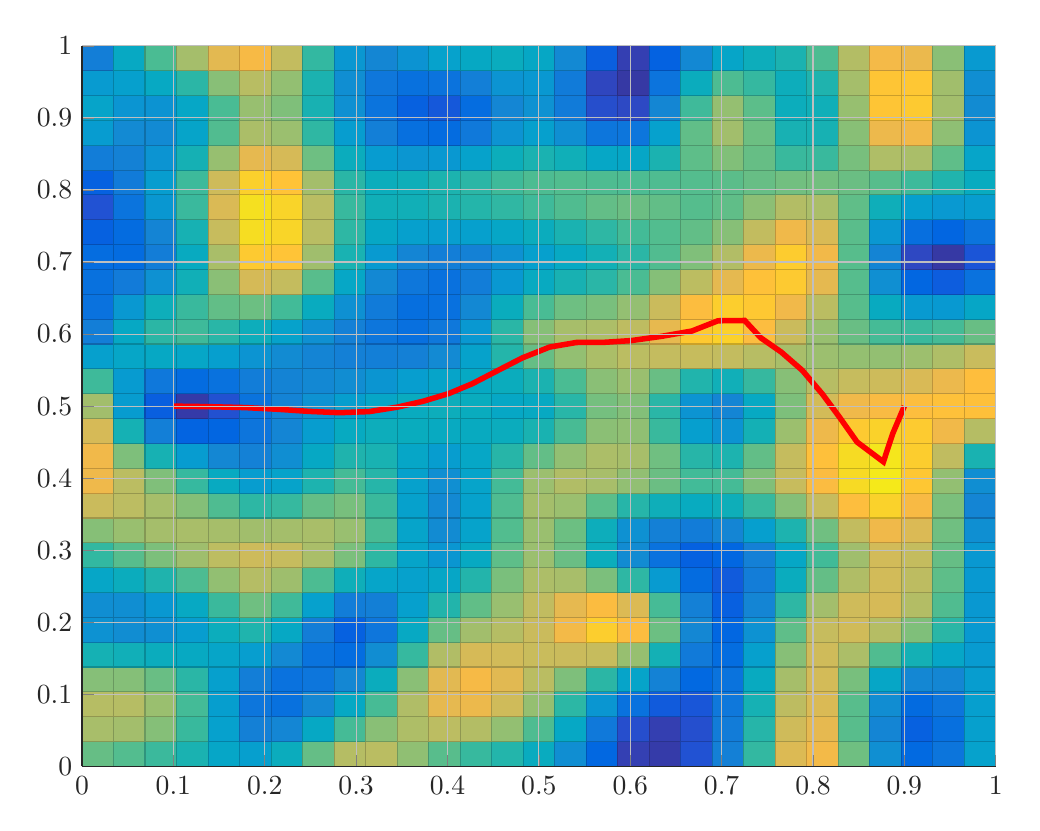
\begin{tikzpicture}

\begin{axis}[%
width=4.56842105263158in,
height=3.60315789473684in,
view={0}{90},
scale only axis,
every outer x axis line/.append style={white!15!black},
every x tick label/.append style={font=\color{white!15!black}},
xmin=0,
xmax=1,
xmajorgrids,
every outer y axis line/.append style={white!15!black},
every y tick label/.append style={font=\color{white!15!black}},
ymin=0,
ymax=1,
ymajorgrids,
every outer z axis line/.append style={white!15!black},
every z tick label/.append style={font=\color{white!15!black}},
zmin=0.00314341829170151,
zmax=3,
ztick={\empty},
zmajorgrids,
axis x line*=bottom,
axis y line*=left,
axis z line*=left
]

\addplot3[%
surf,
shader=faceted,
draw=black,
colormap={mymap}{[1pt] rgb(0pt)=(0.2081,0.1663,0.5292); rgb(1pt)=(0.211624,0.189781,0.577676); rgb(2pt)=(0.212252,0.213771,0.626971); rgb(3pt)=(0.2081,0.2386,0.677086); rgb(4pt)=(0.195905,0.264457,0.7279); rgb(5pt)=(0.170729,0.291938,0.779248); rgb(6pt)=(0.125271,0.324243,0.830271); rgb(7pt)=(0.0591333,0.359833,0.868333); rgb(8pt)=(0.0116952,0.38751,0.881957); rgb(9pt)=(0.00595714,0.408614,0.882843); rgb(10pt)=(0.0165143,0.4266,0.878633); rgb(11pt)=(0.0328524,0.443043,0.871957); rgb(12pt)=(0.0498143,0.458571,0.864057); rgb(13pt)=(0.0629333,0.47369,0.855438); rgb(14pt)=(0.0722667,0.488667,0.8467); rgb(15pt)=(0.0779429,0.503986,0.838371); rgb(16pt)=(0.0793476,0.520024,0.831181); rgb(17pt)=(0.0749429,0.537543,0.826271); rgb(18pt)=(0.0640571,0.556986,0.823957); rgb(19pt)=(0.0487714,0.577224,0.822829); rgb(20pt)=(0.0343429,0.596581,0.819852); rgb(21pt)=(0.0265,0.6137,0.8135); rgb(22pt)=(0.0238905,0.628662,0.803762); rgb(23pt)=(0.0230905,0.641786,0.791267); rgb(24pt)=(0.0227714,0.653486,0.776757); rgb(25pt)=(0.0266619,0.664195,0.760719); rgb(26pt)=(0.0383714,0.674271,0.743552); rgb(27pt)=(0.0589714,0.683757,0.725386); rgb(28pt)=(0.0843,0.692833,0.706167); rgb(29pt)=(0.113295,0.7015,0.685857); rgb(30pt)=(0.145271,0.709757,0.664629); rgb(31pt)=(0.180133,0.717657,0.642433); rgb(32pt)=(0.217829,0.725043,0.619262); rgb(33pt)=(0.258643,0.731714,0.595429); rgb(34pt)=(0.302171,0.737605,0.571186); rgb(35pt)=(0.348167,0.742433,0.547267); rgb(36pt)=(0.395257,0.7459,0.524443); rgb(37pt)=(0.44201,0.748081,0.503314); rgb(38pt)=(0.487124,0.749062,0.483976); rgb(39pt)=(0.530029,0.749114,0.466114); rgb(40pt)=(0.570857,0.748519,0.44939); rgb(41pt)=(0.609852,0.747314,0.433686); rgb(42pt)=(0.6473,0.7456,0.4188); rgb(43pt)=(0.683419,0.743476,0.404433); rgb(44pt)=(0.71841,0.741133,0.390476); rgb(45pt)=(0.752486,0.7384,0.376814); rgb(46pt)=(0.785843,0.735567,0.363271); rgb(47pt)=(0.818505,0.732733,0.34979); rgb(48pt)=(0.850657,0.7299,0.336029); rgb(49pt)=(0.882433,0.727433,0.3217); rgb(50pt)=(0.913933,0.725786,0.306276); rgb(51pt)=(0.944957,0.726114,0.288643); rgb(52pt)=(0.973895,0.731395,0.266648); rgb(53pt)=(0.993771,0.745457,0.240348); rgb(54pt)=(0.999043,0.765314,0.216414); rgb(55pt)=(0.995533,0.786057,0.196652); rgb(56pt)=(0.988,0.8066,0.179367); rgb(57pt)=(0.978857,0.827143,0.163314); rgb(58pt)=(0.9697,0.848138,0.147452); rgb(59pt)=(0.962586,0.870514,0.1309); rgb(60pt)=(0.958871,0.8949,0.113243); rgb(61pt)=(0.959824,0.921833,0.0948381); rgb(62pt)=(0.9661,0.951443,0.0755333); rgb(63pt)=(0.9763,0.9831,0.0538)},
mesh/rows=30]
table[row sep=crcr,header=false] {0	0	0.154906710881439\\
0	0.0344827586206897	0.188671654362867\\
0	0.0689655172413793	0.203260315946722\\
0	0.103448275862069	0.198399476660408\\
0	0.137931034482759	0.159302804294505\\
0	0.172413793103448	0.106384498433381\\
0	0.206896551724138	0.0812709850799054\\
0	0.241379310344828	0.0932460420520926\\
0	0.275862068965517	0.122914827812116\\
0	0.310344827586207	0.155255447885464\\
0	0.344827586206897	0.197256727190997\\
0	0.379310344827586	0.238545177550327\\
0	0.413793103448276	0.26269991668803\\
0	0.448275862068965	0.276365565125784\\
0	0.482758620689655	0.271123291160669\\
0	0.517241379310345	0.229178939025944\\
0	0.551724137931034	0.140591698721558\\
0	0.586206896551724	0.0559813941473222\\
0	0.620689655172414	0.026234016806574\\
0	0.655172413793103	0.0402750643962934\\
0	0.689655172413793	0.0591078171001346\\
0	0.724137931034483	0.0503667527596023\\
0	0.758620689655172	0.0258095826820979\\
0	0.793103448275862	0.0134735591794228\\
0	0.827586206896552	0.0411062490514203\\
0	0.862068965517241	0.0952043743546157\\
0	0.896551724137931	0.128158828995084\\
0	0.931034482758621	0.116371399068031\\
0	0.96551724137931	0.0765284566786142\\
0	1	0.00873947334247309\\
0.0344827586206897	0	0.143357377465235\\
0.0344827586206897	0.0344827586206897	0.188156481887945\\
0.0344827586206897	0.0689655172413793	0.209307334665501\\
0.0344827586206897	0.103448275862069	0.206470408538239\\
0.0344827586206897	0.137931034482759	0.161218195974597\\
0.0344827586206897	0.172413793103448	0.098994319660914\\
0.0344827586206897	0.206896551724138	0.071878723485973\\
0.0344827586206897	0.241379310344828	0.0953638277904553\\
0.0344827586206897	0.275862068965517	0.13858297854722\\
0.0344827586206897	0.310344827586207	0.171882646662074\\
0.0344827586206897	0.344827586206897	0.201339510997754\\
0.0344827586206897	0.379310344827586	0.222346018343874\\
0.0344827586206897	0.413793103448276	0.219857937188229\\
0.0344827586206897	0.448275862068965	0.18864395251805\\
0.0344827586206897	0.482758620689655	0.150251343971767\\
0.0344827586206897	0.517241379310345	0.126856660290881\\
0.0344827586206897	0.551724137931034	0.114807241702754\\
0.0344827586206897	0.586206896551724	0.104417138760706\\
0.0344827586206897	0.620689655172414	0.0878203731230385\\
0.0344827586206897	0.655172413793103	0.066214772719545\\
0.0344827586206897	0.689655172413793	0.0481188936397464\\
0.0344827586206897	0.724137931034483	0.0398466330338348\\
0.0344827586206897	0.758620689655172	0.0385382859908233\\
0.0344827586206897	0.793103448275862	0.0432551844895341\\
0.0344827586206897	0.827586206896552	0.0564717474331274\\
0.0344827586206897	0.862068965517241	0.0774631771055632\\
0.0344827586206897	0.896551724137931	0.0937899351306242\\
0.0344827586206897	0.931034482758621	0.0992163665830521\\
0.0344827586206897	0.96551724137931	0.0981582768399905\\
0.0344827586206897	1	0.0906484808130359\\
0.0689655172413793	0	0.134398461991296\\
0.0689655172413793	0.0344827586206897	0.179711409595783\\
0.0689655172413793	0.0689655172413793	0.201751235431789\\
0.0689655172413793	0.103448275862069	0.200175355576923\\
0.0689655172413793	0.137931034482759	0.156217487581846\\
0.0689655172413793	0.172413793103448	0.0957967926508189\\
0.0689655172413793	0.206896551724138	0.072115402136352\\
0.0689655172413793	0.241379310344828	0.103954404705074\\
0.0689655172413793	0.275862068965517	0.15475836093758\\
0.0689655172413793	0.310344827586207	0.185966378243866\\
0.0689655172413793	0.344827586206897	0.201743067254592\\
0.0689655172413793	0.379310344827586	0.203789277028186\\
0.0689655172413793	0.413793103448276	0.181595882253904\\
0.0689655172413793	0.448275862068965	0.122241219624798\\
0.0689655172413793	0.482758620689655	0.0647096097608859\\
0.0689655172413793	0.517241379310345	0.0554504623272347\\
0.0689655172413793	0.551724137931034	0.0952008218220807\\
0.0689655172413793	0.586206896551724	0.135769288210663\\
0.0689655172413793	0.620689655172414	0.131928747838081\\
0.0689655172413793	0.655172413793103	0.0930624432146233\\
0.0689655172413793	0.689655172413793	0.0561285859462883\\
0.0689655172413793	0.724137931034483	0.050652261264066\\
0.0689655172413793	0.758620689655172	0.0651344744360789\\
0.0689655172413793	0.793103448275862	0.0801996648999252\\
0.0689655172413793	0.827586206896552	0.0813285496611843\\
0.0689655172413793	0.862068965517241	0.0762440737716039\\
0.0689655172413793	0.896551724137931	0.0786510483718057\\
0.0689655172413793	0.931034482758621	0.095247501631704\\
0.0689655172413793	0.96551724137931	0.121307864316802\\
0.0689655172413793	1	0.156807366169713\\
0.103448275862069	0	0.127975996599197\\
0.103448275862069	0.0344827586206897	0.163177731173319\\
0.103448275862069	0.0689655172413793	0.180387830041468\\
0.103448275862069	0.103448275862069	0.179324727967304\\
0.103448275862069	0.137931034482759	0.144229178272906\\
0.103448275862069	0.172413793103448	0.0968821200865302\\
0.103448275862069	0.206896551724138	0.0821540904665596\\
0.103448275862069	0.241379310344828	0.119161471288929\\
0.103448275862069	0.275862068965517	0.171510494619272\\
0.103448275862069	0.310344827586207	0.197518284743681\\
0.103448275862069	0.344827586206897	0.198419776089465\\
0.103448275862069	0.379310344827586	0.182786894614941\\
0.103448275862069	0.413793103448276	0.147854066081868\\
0.103448275862069	0.448275862068965	0.0772250077424967\\
0.103448275862069	0.482758620689655	0.0146871696531805\\
0.103448275862069	0.517241379310345	0.0151404840569755\\
0.103448275862069	0.551724137931034	0.0818031036245468\\
0.103448275862069	0.586206896551724	0.149935040301155\\
0.103448275862069	0.620689655172414	0.158494038370674\\
0.103448275862069	0.655172413793103	0.120935880982913\\
0.103448275862069	0.689655172413793	0.0834274981877612\\
0.103448275862069	0.724137931034483	0.0831101870594358\\
0.103448275862069	0.758620689655172	0.105873116078701\\
0.103448275862069	0.793103448275862	0.124525985133773\\
0.103448275862069	0.827586206896552	0.115893477766413\\
0.103448275862069	0.862068965517241	0.0917838152564211\\
0.103448275862069	0.896551724137931	0.0829800179460326\\
0.103448275862069	0.931034482758621	0.104665132841256\\
0.103448275862069	0.96551724137931	0.146115368626967\\
0.103448275862069	1	0.207267515788863\\
0.137931034482759	0	0.119933980878321\\
0.137931034482759	0.0344827586206897	0.127012900676483\\
0.137931034482759	0.0689655172413793	0.130515422602855\\
0.137931034482759	0.103448275862069	0.130343262732128\\
0.137931034482759	0.137931034482759	0.120195060346046\\
0.137931034482759	0.172413793103448	0.108814910313619\\
0.137931034482759	0.206896551724138	0.114528463369706\\
0.137931034482759	0.241379310344828	0.151464897049834\\
0.137931034482759	0.275862068965517	0.19403386001156\\
0.137931034482759	0.310344827586207	0.207532460401796\\
0.137931034482759	0.344827586206897	0.187966022372406\\
0.137931034482759	0.379310344827586	0.152834448348367\\
0.137931034482759	0.413793103448276	0.113931479364164\\
0.137931034482759	0.448275862068965	0.0576672690685674\\
0.137931034482759	0.482758620689655	0.0127138062795787\\
0.137931034482759	0.517241379310345	0.0179910784718922\\
0.137931034482759	0.551724137931034	0.0766201337915457\\
0.137931034482759	0.586206896551724	0.139997282492416\\
0.137931034482759	0.620689655172414	0.16345016252137\\
0.137931034482759	0.655172413793103	0.158634886010367\\
0.137931034482759	0.689655172413793	0.150934500647195\\
0.137931034482759	0.724137931034483	0.160728574354105\\
0.137931034482759	0.758620689655172	0.180744457656523\\
0.137931034482759	0.793103448275862	0.192339508369921\\
0.137931034482759	0.827586206896552	0.175995563593915\\
0.137931034482759	0.862068965517241	0.141067072573214\\
0.137931034482759	0.896551724137931	0.12370979133062\\
0.137931034482759	0.931034482758621	0.141871298225029\\
0.137931034482759	0.96551724137931	0.18287152854646\\
0.137931034482759	1	0.246633576656987\\
0.172413793103448	0	0.116074131880312\\
0.172413793103448	0.0344827586206897	0.0873101134275105\\
0.172413793103448	0.0689655172413793	0.0726272064247306\\
0.172413793103448	0.103448275862069	0.072151601632695\\
0.172413793103448	0.137931034482759	0.0911631116665623\\
0.172413793103448	0.172413793103448	0.122442350472846\\
0.172413793103448	0.206896551724138	0.151765151813467\\
0.172413793103448	0.241379310344828	0.186252245996029\\
0.172413793103448	0.275862068965517	0.21508172760876\\
0.172413793103448	0.310344827586207	0.214618271984652\\
0.172413793103448	0.344827586206897	0.175125418196635\\
0.172413793103448	0.379310344827586	0.123003850642132\\
0.172413793103448	0.413793103448276	0.0863937807829885\\
0.172413793103448	0.448275862068965	0.0579172587262363\\
0.172413793103448	0.482758620689655	0.0413582055535994\\
0.172413793103448	0.517241379310345	0.0472140657743631\\
0.172413793103448	0.551724137931034	0.0768620219152699\\
0.172413793103448	0.586206896551724	0.115582643570869\\
0.172413793103448	0.620689655172414	0.15244529045666\\
0.172413793103448	0.655172413793103	0.193883123254798\\
0.172413793103448	0.689655172413793	0.229490364220819\\
0.172413793103448	0.724137931034483	0.250738874582848\\
0.172413793103448	0.758620689655172	0.261877471558351\\
0.172413793103448	0.793103448275862	0.261179835364824\\
0.172413793103448	0.827586206896552	0.239563420927091\\
0.172413793103448	0.862068965517241	0.2004204365428\\
0.172413793103448	0.896551724137931	0.17724321080992\\
0.172413793103448	0.931034482758621	0.186791347313158\\
0.172413793103448	0.96551724137931	0.217220968160476\\
0.172413793103448	1	0.268458403548\\
0.206896551724138	0	0.128826750441911\\
0.206896551724138	0.0344827586206897	0.0771466610968231\\
0.206896551724138	0.0689655172413793	0.0484889405352605\\
0.206896551724138	0.103448275862069	0.0430799913567003\\
0.206896551724138	0.137931034482759	0.0710551776845678\\
0.206896551724138	0.172413793103448	0.118517134138273\\
0.206896551724138	0.206896551724138	0.157654025116371\\
0.206896551724138	0.241379310344828	0.193355031728336\\
0.206896551724138	0.275862068965517	0.219798719005357\\
0.206896551724138	0.310344827586207	0.216078294757634\\
0.206896551724138	0.344827586206897	0.169853417859041\\
0.206896551724138	0.379310344827586	0.11218280183241\\
0.206896551724138	0.413793103448276	0.0790958258605906\\
0.206896551724138	0.448275862068965	0.0669887833256247\\
0.206896551724138	0.482758620689655	0.0656144757481972\\
0.206896551724138	0.517241379310345	0.0689618370080776\\
0.206896551724138	0.551724137931034	0.0768784726618812\\
0.206896551724138	0.586206896551724	0.0960337022697134\\
0.206896551724138	0.620689655172414	0.136623324538811\\
0.206896551724138	0.655172413793103	0.201385992185221\\
0.206896551724138	0.689655172413793	0.259488902859344\\
0.206896551724138	0.724137931034483	0.286125900338996\\
0.206896551724138	0.758620689655172	0.29208978287232\\
0.206896551724138	0.793103448275862	0.284793838452262\\
0.206896551724138	0.827586206896552	0.26123209543701\\
0.206896551724138	0.862068965517241	0.221432615638151\\
0.206896551724138	0.896551724137931	0.195429713206975\\
0.206896551724138	0.931034482758621	0.19832852428018\\
0.206896551724138	0.96551724137931	0.219450168676177\\
0.206896551724138	1	0.258725755779871\\
0.241379310344828	0	0.174028912946745\\
0.241379310344828	0.0344827586206897	0.112684239911681\\
0.241379310344828	0.0689655172413793	0.0716545676878972\\
0.241379310344828	0.103448275862069	0.0510848276064048\\
0.241379310344828	0.137931034482759	0.0558101383986529\\
0.241379310344828	0.172413793103448	0.0792909560332317\\
0.241379310344828	0.206896551724138	0.108840386206046\\
0.241379310344828	0.241379310344828	0.15544383327585\\
0.241379310344828	0.275862068965517	0.201642727927409\\
0.241379310344828	0.310344827586207	0.213639287067834\\
0.241379310344828	0.344827586206897	0.180941067594915\\
0.241379310344828	0.379310344827586	0.134260514049241\\
0.241379310344828	0.413793103448276	0.105811053096054\\
0.241379310344828	0.448275862068965	0.0917973442303853\\
0.241379310344828	0.482758620689655	0.0844829454543074\\
0.241379310344828	0.517241379310345	0.0796121173501732\\
0.241379310344828	0.551724137931034	0.0755815321351691\\
0.241379310344828	0.586206896551724	0.0821341633185192\\
0.241379310344828	0.620689655172414	0.112320939424468\\
0.241379310344828	0.655172413793103	0.167531372020586\\
0.241379310344828	0.689655172413793	0.218144160418841\\
0.241379310344828	0.724137931034483	0.240674513178951\\
0.241379310344828	0.758620689655172	0.24542829353762\\
0.241379310344828	0.793103448275862	0.238840567743729\\
0.241379310344828	0.827586206896552	0.218827502926597\\
0.241379310344828	0.862068965517241	0.185249951434871\\
0.241379310344828	0.896551724137931	0.16157489438668\\
0.241379310344828	0.931034482758621	0.159606781591191\\
0.241379310344828	0.96551724137931	0.170993972949854\\
0.241379310344828	1	0.19567892537865\\
0.275862068965517	0	0.223545207962017\\
0.275862068965517	0.0344827586206897	0.163333440891627\\
0.275862068965517	0.0689655172413793	0.115179696657941\\
0.275862068965517	0.103448275862069	0.0790788149529958\\
0.275862068965517	0.137931034482759	0.0510714027397201\\
0.275862068965517	0.172413793103448	0.0367900433796835\\
0.275862068965517	0.206896551724138	0.0484666344074179\\
0.275862068965517	0.241379310344828	0.104831088224831\\
0.275862068965517	0.275862068965517	0.173125891109203\\
0.275862068965517	0.310344827586207	0.204599680020682\\
0.275862068965517	0.344827586206897	0.19248470775747\\
0.275862068965517	0.379310344827586	0.163826993091194\\
0.275862068965517	0.413793103448276	0.141796573515389\\
0.275862068965517	0.448275862068965	0.121585891474497\\
0.275862068965517	0.482758620689655	0.10291604330637\\
0.275862068965517	0.517241379310345	0.0884768427581241\\
0.275862068965517	0.551724137931034	0.0753513118967526\\
0.275862068965517	0.586206896551724	0.0707569449296084\\
0.275862068965517	0.620689655172414	0.0847414884268018\\
0.275862068965517	0.655172413793103	0.11783963185626\\
0.275862068965517	0.689655172413793	0.149777462179112\\
0.275862068965517	0.724137931034483	0.165232687483112\\
0.275862068965517	0.758620689655172	0.171385367255895\\
0.275862068965517	0.793103448275862	0.169055836162834\\
0.275862068965517	0.827586206896552	0.154313185037836\\
0.275862068965517	0.862068965517241	0.128463038753057\\
0.275862068965517	0.896551724137931	0.108567970838777\\
0.275862068965517	0.931034482758621	0.103172193726323\\
0.275862068965517	0.96551724137931	0.106222056733341\\
0.275862068965517	1	0.117670792355515\\
0.310344827586207	0	0.235829505321182\\
0.310344827586207	0.0344827586206897	0.192306746374361\\
0.310344827586207	0.0689655172413793	0.152112797513791\\
0.310344827586207	0.103448275862069	0.115142839724961\\
0.310344827586207	0.137931034482759	0.0725605260561982\\
0.310344827586207	0.172413793103448	0.0367082817792361\\
0.310344827586207	0.206896551724138	0.0334049495816032\\
0.310344827586207	0.241379310344828	0.0823524406707524\\
0.310344827586207	0.275862068965517	0.147941086740759\\
0.310344827586207	0.310344827586207	0.182150134127008\\
0.310344827586207	0.344827586206897	0.181056743178021\\
0.310344827586207	0.379310344827586	0.16565452175861\\
0.310344827586207	0.413793103448276	0.151350945699406\\
0.310344827586207	0.448275862068965	0.134551147228165\\
0.310344827586207	0.482758620689655	0.116047184178093\\
0.310344827586207	0.517241379310345	0.0982410942294163\\
0.310344827586207	0.551724137931034	0.0778341484608628\\
0.310344827586207	0.586206896551724	0.0635428654247094\\
0.310344827586207	0.620689655172414	0.0657177900340259\\
0.310344827586207	0.655172413793103	0.0832805346109423\\
0.310344827586207	0.689655172413793	0.102934400736691\\
0.310344827586207	0.724137931034483	0.116272634017421\\
0.310344827586207	0.758620689655172	0.128211126780606\\
0.310344827586207	0.793103448275862	0.131907697588538\\
0.310344827586207	0.827586206896552	0.118272894765191\\
0.310344827586207	0.862068965517241	0.0915058539650255\\
0.310344827586207	0.896551724137931	0.0707924552664331\\
0.310344827586207	0.931034482758621	0.0656689663125671\\
0.310344827586207	0.96551724137931	0.0693746432887008\\
0.310344827586207	1	0.0818547888382275\\
0.344827586206897	0	0.199949072939981\\
0.344827586206897	0.0344827586206897	0.198523446488192\\
0.344827586206897	0.0689655172413793	0.188828083146083\\
0.344827586206897	0.103448275862069	0.17070256331366\\
0.344827586206897	0.137931034482759	0.134584263507016\\
0.344827586206897	0.172413793103448	0.093715212757748\\
0.344827586206897	0.206896551724138	0.0753658579243527\\
0.344827586206897	0.241379310344828	0.0911984891251125\\
0.344827586206897	0.275862068965517	0.119049977343962\\
0.344827586206897	0.310344827586207	0.133202775842753\\
0.344827586206897	0.344827586206897	0.131823861794095\\
0.344827586206897	0.379310344827586	0.125640814112672\\
0.344827586206897	0.413793103448276	0.122925926369726\\
0.344827586206897	0.448275862068965	0.124940034232472\\
0.344827586206897	0.482758620689655	0.123871100871236\\
0.344827586206897	0.517241379310345	0.11051007780302\\
0.344827586206897	0.551724137931034	0.082309173118662\\
0.344827586206897	0.586206896551724	0.0568585796351116\\
0.344827586206897	0.620689655172414	0.0508640397140147\\
0.344827586206897	0.655172413793103	0.0599437341101855\\
0.344827586206897	0.689655172413793	0.0748530326903734\\
0.344827586206897	0.724137931034483	0.0930213332510682\\
0.344827586206897	0.758620689655172	0.118178834383435\\
0.344827586206897	0.793103448275862	0.131549976918225\\
0.344827586206897	0.827586206896552	0.113140912619852\\
0.344827586206897	0.862068965517241	0.0726634684557812\\
0.344827586206897	0.896551724137931	0.0443809150884882\\
0.344827586206897	0.931034482758621	0.045270146521633\\
0.344827586206897	0.96551724137931	0.0633055032919612\\
0.344827586206897	1	0.0983956122954372\\
0.379310344827586	0	0.15002107617558\\
0.379310344827586	0.0344827586206897	0.194290734960103\\
0.379310344827586	0.0689655172413793	0.219424524530341\\
0.379310344827586	0.103448275862069	0.225231187163516\\
0.379310344827586	0.137931034482759	0.20306008677511\\
0.379310344827586	0.172413793103448	0.164777588868745\\
0.379310344827586	0.206896551724138	0.134420863042859\\
0.379310344827586	0.241379310344828	0.113565527604172\\
0.379310344827586	0.275862068965517	0.0973687455994111\\
0.379310344827586	0.310344827586207	0.0868761328764229\\
0.379310344827586	0.344827586206897	0.0820842241996374\\
0.379310344827586	0.379310344827586	0.0827893873844605\\
0.379310344827586	0.413793103448276	0.0903348362112463\\
0.379310344827586	0.448275862068965	0.110693364323997\\
0.379310344827586	0.482758620689655	0.12772454202438\\
0.379310344827586	0.517241379310345	0.121203479324099\\
0.379310344827586	0.551724137931034	0.0898311597017354\\
0.379310344827586	0.586206896551724	0.0578319293498248\\
0.379310344827586	0.620689655172414	0.0460878555207731\\
0.379310344827586	0.655172413793103	0.0475080001105447\\
0.379310344827586	0.689655172413793	0.0580088692200145\\
0.379310344827586	0.724137931034483	0.0816438044356332\\
0.379310344827586	0.758620689655172	0.120625220881249\\
0.379310344827586	0.793103448275862	0.143892402034668\\
0.379310344827586	0.827586206896552	0.120017316020835\\
0.379310344827586	0.862068965517241	0.0644518104757275\\
0.379310344827586	0.896551724137931	0.0279867040021091\\
0.379310344827586	0.931034482758621	0.0357632981309153\\
0.379310344827586	0.96551724137931	0.0699800837330883\\
0.379310344827586	1	0.130506158654379\\
0.413793103448276	0	0.121521363239092\\
0.413793103448276	0.0344827586206897	0.186918817583993\\
0.413793103448276	0.0689655172413793	0.22920651143412\\
0.413793103448276	0.103448275862069	0.248190256809666\\
0.413793103448276	0.137931034482759	0.236178866521793\\
0.413793103448276	0.172413793103448	0.203663586092488\\
0.413793103448276	0.206896551724138	0.17169837161932\\
0.413793103448276	0.241379310344828	0.137258522110069\\
0.413793103448276	0.275862068965517	0.103533576688783\\
0.413793103448276	0.310344827586207	0.0835081139545166\\
0.413793103448276	0.344827586206897	0.0786189451974982\\
0.413793103448276	0.379310344827586	0.0824773066061422\\
0.413793103448276	0.413793103448276	0.0910717243085744\\
0.413793103448276	0.448275862068965	0.110338159887314\\
0.413793103448276	0.482758620689655	0.127171683679891\\
0.413793103448276	0.517241379310345	0.124609133563022\\
0.413793103448276	0.551724137931034	0.102527644359303\\
0.413793103448276	0.586206896551724	0.0779941746179747\\
0.413793103448276	0.620689655172414	0.0641535647597216\\
0.413793103448276	0.655172413793103	0.0548044193424312\\
0.413793103448276	0.689655172413793	0.0554947032906212\\
0.413793103448276	0.724137931034483	0.0785407004147697\\
0.413793103448276	0.758620689655172	0.123100379841817\\
0.413793103448276	0.793103448275862	0.151466638115429\\
0.413793103448276	0.827586206896552	0.127280396174905\\
0.413793103448276	0.862068965517241	0.0686371527003311\\
0.413793103448276	0.896551724137931	0.0305149792413832\\
0.413793103448276	0.931034482758621	0.0400925265270236\\
0.413793103448276	0.96551724137931	0.0781248468369742\\
0.413793103448276	1	0.144469908011192\\
0.448275862068965	0	0.114167814333664\\
0.448275862068965	0.0344827586206897	0.176636587443154\\
0.448275862068965	0.0689655172413793	0.218882923010149\\
0.448275862068965	0.103448275862069	0.240732594378929\\
0.448275862068965	0.137931034482759	0.235134039745672\\
0.448275862068965	0.172413793103448	0.211715331991715\\
0.448275862068965	0.206896551724138	0.189884468463938\\
0.448275862068965	0.241379310344828	0.168647703681614\\
0.448275862068965	0.275862068965517	0.147900505050378\\
0.448275862068965	0.310344827586207	0.134830841973146\\
0.448275862068965	0.344827586206897	0.131514840791986\\
0.448275862068965	0.379310344827586	0.131749835490685\\
0.448275862068965	0.413793103448276	0.128947891654814\\
0.448275862068965	0.448275862068965	0.12312279611529\\
0.448275862068965	0.482758620689655	0.117848095699046\\
0.448275862068965	0.517241379310345	0.116898099341967\\
0.448275862068965	0.551724137931034	0.121625347597734\\
0.448275862068965	0.586206896551724	0.123765550407976\\
0.448275862068965	0.620689655172414	0.112710490113027\\
0.448275862068965	0.655172413793103	0.0877672810058033\\
0.448275862068965	0.689655172413793	0.071143034294304\\
0.448275862068965	0.724137931034483	0.0867576293888954\\
0.448275862068965	0.758620689655172	0.128348443164647\\
0.448275862068965	0.793103448275862	0.15732774161488\\
0.448275862068965	0.827586206896552	0.139416143314129\\
0.448275862068965	0.862068965517241	0.0920515221930611\\
0.448275862068965	0.896551724137931	0.060462926071268\\
0.448275862068965	0.931034482758621	0.0669419219953507\\
0.448275862068965	0.96551724137931	0.0956965628526433\\
0.448275862068965	1	0.146605907065156\\
0.482758620689655	0	0.1091396757481\\
0.482758620689655	0.0344827586206897	0.158806629783346\\
0.482758620689655	0.0689655172413793	0.19469078972649\\
0.482758620689655	0.103448275862069	0.216672160353807\\
0.482758620689655	0.137931034482759	0.219851607974783\\
0.482758620689655	0.172413793103448	0.210920885313934\\
0.482758620689655	0.206896551724138	0.203430586312908\\
0.482758620689655	0.241379310344828	0.197925078253655\\
0.482758620689655	0.275862068965517	0.192225844914733\\
0.482758620689655	0.310344827586207	0.188173289685813\\
0.482758620689655	0.344827586206897	0.188821517500689\\
0.482758620689655	0.379310344827586	0.187324605597706\\
0.482758620689655	0.413793103448276	0.173417210526706\\
0.482758620689655	0.448275862068965	0.140792138946229\\
0.482758620689655	0.482758620689655	0.111321670121385\\
0.482758620689655	0.517241379310345	0.111156199124761\\
0.482758620689655	0.551724137931034	0.14277204673709\\
0.482758620689655	0.586206896551724	0.17213693537111\\
0.482758620689655	0.620689655172414	0.164883219082096\\
0.482758620689655	0.655172413793103	0.126142760393277\\
0.482758620689655	0.689655172413793	0.0933187556602596\\
0.482758620689655	0.724137931034483	0.100388231645055\\
0.482758620689655	0.758620689655172	0.136118779584325\\
0.482758620689655	0.793103448275862	0.163180126032232\\
0.482758620689655	0.827586206896552	0.151192939053225\\
0.482758620689655	0.862068965517241	0.115998255716251\\
0.482758620689655	0.896551724137931	0.0908784594143177\\
0.482758620689655	0.931034482758621	0.0921568313200477\\
0.482758620689655	0.96551724137931	0.108259002806943\\
0.482758620689655	1	0.139090174400812\\
0.517241379310345	0	0.0893923843416206\\
0.517241379310345	0.0344827586206897	0.126514687073802\\
0.517241379310345	0.0689655172413793	0.158007834092696\\
0.517241379310345	0.103448275862069	0.183868745990157\\
0.517241379310345	0.137931034482759	0.205536317144829\\
0.517241379310345	0.172413793103448	0.220951486972591\\
0.517241379310345	0.206896551724138	0.225672169329098\\
0.517241379310345	0.241379310344828	0.213327942715937\\
0.517241379310345	0.275862068965517	0.195065459483449\\
0.517241379310345	0.310344827586207	0.187800009354195\\
0.517241379310345	0.344827586206897	0.197440811891066\\
0.517241379310345	0.379310344827586	0.207163400244175\\
0.517241379310345	0.413793103448276	0.196821674782915\\
0.517241379310345	0.448275862068965	0.159276642649118\\
0.517241379310345	0.482758620689655	0.123921503732231\\
0.517241379310345	0.517241379310345	0.124242969155159\\
0.517241379310345	0.551724137931034	0.162495518303996\\
0.517241379310345	0.586206896551724	0.198148376954318\\
0.517241379310345	0.620689655172414	0.191034147610338\\
0.517241379310345	0.655172413793103	0.14769078332476\\
0.517241379310345	0.689655172413793	0.10929165074845\\
0.517241379310345	0.724137931034483	0.112382853636039\\
0.517241379310345	0.758620689655172	0.144508848471888\\
0.517241379310345	0.793103448275862	0.168289620678204\\
0.517241379310345	0.827586206896552	0.153861166648457\\
0.517241379310345	0.862068965517241	0.116874845167122\\
0.517241379310345	0.896551724137931	0.0886179234215893\\
0.517241379310345	0.931034482758621	0.0844141490849026\\
0.517241379310345	0.96551724137931	0.0933927125265157\\
0.517241379310345	1	0.115461544845133\\
0.551724137931034	0	0.0537844529420605\\
0.551724137931034	0.0344827586206897	0.07396246335017\\
0.551724137931034	0.0689655172413793	0.100820114373584\\
0.551724137931034	0.103448275862069	0.13456513011162\\
0.551724137931034	0.137931034482759	0.188772594671411\\
0.551724137931034	0.172413793103448	0.244595267868492\\
0.551724137931034	0.206896551724138	0.26291116097753\\
0.551724137931034	0.241379310344828	0.220622625029438\\
0.551724137931034	0.275862068965517	0.160311922133607\\
0.551724137931034	0.310344827586207	0.137107814191537\\
0.551724137931034	0.344827586206897	0.162015536097959\\
0.551724137931034	0.379310344827586	0.197408540001056\\
0.551724137931034	0.413793103448276	0.205731762188437\\
0.551724137931034	0.448275862068965	0.184503494721051\\
0.551724137931034	0.482758620689655	0.160578381738679\\
0.551724137931034	0.517241379310345	0.160291815082386\\
0.551724137931034	0.551724137931034	0.184133087941463\\
0.551724137931034	0.586206896551724	0.204457285228503\\
0.551724137931034	0.620689655172414	0.193474575737456\\
0.551724137931034	0.655172413793103	0.154700481849955\\
0.551724137931034	0.689655172413793	0.121312452228238\\
0.551724137931034	0.724137931034483	0.124728468182292\\
0.551724137931034	0.758620689655172	0.155145364680616\\
0.551724137931034	0.793103448275862	0.173602458676249\\
0.551724137931034	0.827586206896552	0.147068885127715\\
0.551724137931034	0.862068965517241	0.0925499898574339\\
0.551724137931034	0.896551724137931	0.0499276507135547\\
0.551724137931034	0.931034482758621	0.0388120370157684\\
0.551724137931034	0.96551724137931	0.0452966996749041\\
0.551724137931034	1	0.0692668913979473\\
0.586206896551724	0	0.0231886741121234\\
0.586206896551724	0.0344827586206897	0.0275824265026093\\
0.586206896551724	0.0689655172413793	0.0487347420694131\\
0.586206896551724	0.103448275862069	0.0870245776092002\\
0.586206896551724	0.137931034482759	0.165860446591071\\
0.586206896551724	0.172413793103448	0.252793424560162\\
0.586206896551724	0.206896551724138	0.280580332450574\\
0.586206896551724	0.241379310344828	0.212113467722333\\
0.586206896551724	0.275862068965517	0.116226929854743\\
0.586206896551724	0.310344827586207	0.0803037029691965\\
0.586206896551724	0.344827586206897	0.119924373912845\\
0.586206896551724	0.379310344827586	0.17934482160441\\
0.586206896551724	0.413793103448276	0.205631125117206\\
0.586206896551724	0.448275862068965	0.200568412456337\\
0.586206896551724	0.482758620689655	0.188374498993262\\
0.586206896551724	0.517241379310345	0.188540974532132\\
0.586206896551724	0.551724137931034	0.199906634507375\\
0.586206896551724	0.586206896551724	0.207032858012108\\
0.586206896551724	0.620689655172414	0.194012943675699\\
0.586206896551724	0.655172413793103	0.161673057741101\\
0.586206896551724	0.689655172413793	0.13451932822827\\
0.586206896551724	0.724137931034483	0.137778170918657\\
0.586206896551724	0.758620689655172	0.164450257287029\\
0.586206896551724	0.793103448275862	0.176662104824769\\
0.586206896551724	0.827586206896552	0.140737460969946\\
0.586206896551724	0.862068965517241	0.0737743666248206\\
0.586206896551724	0.896551724137931	0.0205528534355869\\
0.586206896551724	0.931034482758621	0.00314341829170151\\
0.586206896551724	0.96551724137931	0.0058974151599564\\
0.586206896551724	1	0.0286872000980963\\
0.620689655172414	0	0.0145081112274505\\
0.620689655172414	0.0344827586206897	0.0112024389747776\\
0.620689655172414	0.0689655172413793	0.0252389350073229\\
0.620689655172414	0.103448275862069	0.0569839777837817\\
0.620689655172414	0.137931034482759	0.128730422389196\\
0.620689655172414	0.172413793103448	0.209589278825035\\
0.620689655172414	0.206896551724138	0.235528180591317\\
0.620689655172414	0.241379310344828	0.170912067452922\\
0.620689655172414	0.275862068965517	0.0818137803034929\\
0.620689655172414	0.310344827586207	0.0525230296752582\\
0.620689655172414	0.344827586206897	0.0999818540188839\\
0.620689655172414	0.379310344827586	0.166462292423983\\
0.620689655172414	0.413793103448276	0.195103476393267\\
0.620689655172414	0.448275862068965	0.185769402761974\\
0.620689655172414	0.482758620689655	0.169768978903579\\
0.620689655172414	0.517241379310345	0.174712589802309\\
0.620689655172414	0.551724137931034	0.19967917317906\\
0.620689655172414	0.586206896551724	0.220435111565824\\
0.620689655172414	0.620689655172414	0.213482562981715\\
0.620689655172414	0.655172413793103	0.18209327384005\\
0.620689655172414	0.689655172413793	0.152873698293727\\
0.620689655172414	0.724137931034483	0.150606616417492\\
0.620689655172414	0.758620689655172	0.167382672738049\\
0.620689655172414	0.793103448275862	0.173707681869287\\
0.620689655172414	0.827586206896552	0.144555423401273\\
0.620689655172414	0.862068965517241	0.0927894147239065\\
0.620689655172414	0.896551724137931	0.0488345129410071\\
0.620689655172414	0.931034482758621	0.0276508690339478\\
0.620689655172414	0.96551724137931	0.0186205747852964\\
0.620689655172414	1	0.0216507547467578\\
0.655172413793103	0	0.0205356350506763\\
0.655172413793103	0.0344827586206897	0.0159534739027155\\
0.655172413793103	0.0689655172413793	0.0209335010018662\\
0.655172413793103	0.103448275862069	0.0356670586013851\\
0.655172413793103	0.137931034482759	0.0716464868079304\\
0.655172413793103	0.172413793103448	0.112954029089431\\
0.655172413793103	0.206896551724138	0.126472219662142\\
0.655172413793103	0.241379310344828	0.0915228440470438\\
0.655172413793103	0.275862068965517	0.0461147833479257\\
0.655172413793103	0.310344827586207	0.0407764929148689\\
0.655172413793103	0.344827586206897	0.0911933417944032\\
0.655172413793103	0.379310344827586	0.151301869929245\\
0.655172413793103	0.413793103448276	0.169772625182187\\
0.655172413793103	0.448275862068965	0.139170684718059\\
0.655172413793103	0.482758620689655	0.10662025088666\\
0.655172413793103	0.517241379310345	0.121122379226243\\
0.655172413793103	0.551724137931034	0.183701635868707\\
0.655172413793103	0.586206896551724	0.242603240513805\\
0.655172413793103	0.620689655172414	0.249368013522617\\
0.655172413793103	0.655172413793103	0.214295830801939\\
0.655172413793103	0.689655172413793	0.175684736994061\\
0.655172413793103	0.724137931034483	0.162876521684775\\
0.655172413793103	0.758620689655172	0.163719681682169\\
0.655172413793103	0.793103448275862	0.164193146886145\\
0.655172413793103	0.827586206896552	0.156880286955784\\
0.655172413793103	0.862068965517241	0.146232552693145\\
0.655172413793103	0.896551724137931	0.129859790121885\\
0.655172413793103	0.931034482758621	0.106435952916059\\
0.655172413793103	0.96551724137931	0.0768662970591563\\
0.655172413793103	1	0.0411377626098597\\
0.689655172413793	0	0.0446053000645701\\
0.689655172413793	0.0344827586206897	0.0404593371696299\\
0.689655172413793	0.0689655172413793	0.0375516868268251\\
0.689655172413793	0.103448275862069	0.0358966374712455\\
0.689655172413793	0.137931034482759	0.036196786103365\\
0.689655172413793	0.172413793103448	0.0374853148447232\\
0.689655172413793	0.206896551724138	0.0375104758640563\\
0.689655172413793	0.241379310344828	0.0303397387923749\\
0.689655172413793	0.275862068965517	0.0262755651515491\\
0.689655172413793	0.310344827586207	0.0425769597959276\\
0.689655172413793	0.344827586206897	0.0931242321661476\\
0.689655172413793	0.379310344827586	0.144525205942696\\
0.689655172413793	0.413793103448276	0.152772844831146\\
0.689655172413793	0.448275862068965	0.104436404624398\\
0.689655172413793	0.482758620689655	0.0581150101001707\\
0.689655172413793	0.517241379310345	0.0789007677891687\\
0.689655172413793	0.551724137931034	0.169126344996404\\
0.689655172413793	0.586206896551724	0.256867601513301\\
0.689655172413793	0.620689655172414	0.275787957966362\\
0.689655172413793	0.655172413793103	0.24170596216234\\
0.689655172413793	0.689655172413793	0.199034239590547\\
0.689655172413793	0.724137931034483	0.177850923031681\\
0.689655172413793	0.758620689655172	0.16363111662493\\
0.689655172413793	0.793103448275862	0.157489930813089\\
0.689655172413793	0.827586206896552	0.16790490431967\\
0.689655172413793	0.862068965517241	0.191580238811444\\
0.689655172413793	0.896551724137931	0.19926801587841\\
0.689655172413793	0.931034482758621	0.176336399866052\\
0.689655172413793	0.96551724137931	0.133110705208455\\
0.689655172413793	1	0.0696464382381828\\
0.724137931034483	0	0.103224741499765\\
0.724137931034483	0.0344827586206897	0.0981830318499006\\
0.724137931034483	0.0689655172413793	0.0911272080045417\\
0.724137931034483	0.103448275862069	0.0820143603411456\\
0.724137931034483	0.137931034482759	0.068228732320875\\
0.724137931034483	0.172413793103448	0.0533949106049818\\
0.724137931034483	0.206896551724138	0.0446965879131844\\
0.724137931034483	0.241379310344828	0.0398164086491667\\
0.724137931034483	0.275862068965517	0.0420995045084127\\
0.724137931034483	0.310344827586207	0.0610291630561657\\
0.724137931034483	0.344827586206897	0.109721353551032\\
0.724137931034483	0.379310344827586	0.158470732851939\\
0.724137931034483	0.413793103448276	0.166545063082963\\
0.724137931034483	0.448275862068965	0.12165219031982\\
0.724137931034483	0.482758620689655	0.0776568180236512\\
0.724137931034483	0.517241379310345	0.0937085451126676\\
0.724137931034483	0.551724137931034	0.170519677809747\\
0.724137931034483	0.586206896551724	0.247456050459635\\
0.724137931034483	0.620689655172414	0.270355464817394\\
0.724137931034483	0.655172413793103	0.253721949501308\\
0.724137931034483	0.689655172413793	0.226404422420258\\
0.724137931034483	0.724137931034483	0.205218778826418\\
0.724137931034483	0.758620689655172	0.180607850904121\\
0.724137931034483	0.793103448275862	0.163829410089722\\
0.724137931034483	0.827586206896552	0.168995722287605\\
0.724137931034483	0.862068965517241	0.189427380471726\\
0.724137931034483	0.896551724137931	0.197657181971243\\
0.724137931034483	0.931034482758621	0.180041886522455\\
0.724137931034483	0.96551724137931	0.146228470499035\\
0.724137931034483	1	0.0962801309021978\\
0.758620689655172	0	0.197414524371232\\
0.758620689655172	0.0344827586206897	0.191716590294144\\
0.758620689655172	0.0689655172413793	0.183144626639287\\
0.758620689655172	0.103448275862069	0.171664646531789\\
0.758620689655172	0.137931034482759	0.15558439827359\\
0.758620689655172	0.172413793103448	0.137233571980093\\
0.758620689655172	0.206896551724138	0.121038780523053\\
0.758620689655172	0.241379310344828	0.101621003084678\\
0.758620689655172	0.275862068965517	0.0877538125171159\\
0.758620689655172	0.310344827586207	0.0965555899724201\\
0.758620689655172	0.344827586206897	0.140766952318611\\
0.758620689655172	0.379310344827586	0.189439516500255\\
0.758620689655172	0.413793103448276	0.2035183193862\\
0.758620689655172	0.448275862068965	0.176902237332173\\
0.758620689655172	0.482758620689655	0.146550467254831\\
0.758620689655172	0.517241379310345	0.149376006843514\\
0.758620689655172	0.551724137931034	0.182230708151241\\
0.758620689655172	0.586206896551724	0.219291163370874\\
0.758620689655172	0.620689655172414	0.241252284274806\\
0.758620689655172	0.655172413793103	0.256389450331484\\
0.758620689655172	0.689655172413793	0.260491554471539\\
0.758620689655172	0.724137931034483	0.245364108620907\\
0.758620689655172	0.758620689655172	0.212311619427998\\
0.758620689655172	0.793103448275862	0.18053801385695\\
0.758620689655172	0.827586206896552	0.16313940432419\\
0.758620689655172	0.862068965517241	0.152740684257733\\
0.758620689655172	0.896551724137931	0.144725873217996\\
0.758620689655172	0.931034482758621	0.136971688246107\\
0.758620689655172	0.96551724137931	0.131010035020846\\
0.758620689655172	1	0.126868872324605\\
0.793103448275862	0	0.259287245549505\\
0.793103448275862	0.0344827586206897	0.25233339480439\\
0.793103448275862	0.0689655172413793	0.243929520904301\\
0.793103448275862	0.103448275862069	0.234080888596759\\
0.793103448275862	0.137931034482759	0.223612188728995\\
0.793103448275862	0.172413793103448	0.211360470578918\\
0.793103448275862	0.206896551724138	0.194526755805995\\
0.793103448275862	0.241379310344828	0.163945120117797\\
0.793103448275862	0.275862068965517	0.135439769225072\\
0.793103448275862	0.310344827586207	0.134675963990328\\
0.793103448275862	0.344827586206897	0.173566823876232\\
0.793103448275862	0.379310344827586	0.220598018898326\\
0.793103448275862	0.413793103448276	0.239462046961685\\
0.793103448275862	0.448275862068965	0.22987345992955\\
0.793103448275862	0.482758620689655	0.212271830607222\\
0.793103448275862	0.517241379310345	0.202396912811038\\
0.793103448275862	0.551724137931034	0.194116972832421\\
0.793103448275862	0.586206896551724	0.192424058735452\\
0.793103448275862	0.620689655172414	0.207861581067049\\
0.793103448275862	0.655172413793103	0.242377175836534\\
0.793103448275862	0.689655172413793	0.268096212936827\\
0.793103448275862	0.724137931034483	0.260045534743459\\
0.793103448275862	0.758620689655172	0.227341609656194\\
0.793103448275862	0.793103448275862	0.190647863278931\\
0.793103448275862	0.827586206896552	0.159102374179601\\
0.793103448275862	0.862068965517241	0.126579433178225\\
0.793103448275862	0.896551724137931	0.107248496900596\\
0.793103448275862	0.931034482758621	0.108407431918882\\
0.793103448275862	0.96551724137931	0.124943574700288\\
0.793103448275862	1	0.156851335362305\\
0.827586206896552	0	0.226523456382098\\
0.827586206896552	0.0344827586206897	0.215999858798129\\
0.827586206896552	0.0689655172413793	0.209615735297695\\
0.827586206896552	0.103448275862069	0.207447878885449\\
0.827586206896552	0.137931034482759	0.214018505211572\\
0.827586206896552	0.172413793103448	0.223067676529242\\
0.827586206896552	0.206896551724138	0.22144808106679\\
0.827586206896552	0.241379310344828	0.198631991234833\\
0.827586206896552	0.275862068965517	0.173662508942565\\
0.827586206896552	0.310344827586207	0.173381528048984\\
0.827586206896552	0.344827586206897	0.208018210138958\\
0.827586206896552	0.379310344827586	0.249198949393125\\
0.827586206896552	0.413793103448276	0.265506781197061\\
0.827586206896552	0.448275862068965	0.25803844430272\\
0.827586206896552	0.482758620689655	0.240982565459401\\
0.827586206896552	0.517241379310345	0.223306328356631\\
0.827586206896552	0.551724137931034	0.198921633702137\\
0.827586206896552	0.586206896551724	0.179308686385044\\
0.827586206896552	0.620689655172414	0.179104653256753\\
0.827586206896552	0.655172413793103	0.197017876733381\\
0.827586206896552	0.689655172413793	0.213027353495702\\
0.827586206896552	0.724137931034483	0.210550035608724\\
0.827586206896552	0.758620689655172	0.196133656921528\\
0.827586206896552	0.793103448275862	0.179939068429098\\
0.827586206896552	0.827586206896552	0.165961935881351\\
0.827586206896552	0.862068965517241	0.151399139975968\\
0.827586206896552	0.896551724137931	0.144732143556514\\
0.827586206896552	0.931034482758621	0.150307182995376\\
0.827586206896552	0.96551724137931	0.165079703559364\\
0.827586206896552	1	0.189046545808953\\
0.862068965517241	0	0.130980252018346\\
0.862068965517241	0.0344827586206897	0.115322508894821\\
0.862068965517241	0.0689655172413793	0.112874792181509\\
0.862068965517241	0.103448275862069	0.123821459192705\\
0.862068965517241	0.137931034482759	0.158047277788774\\
0.862068965517241	0.172413793103448	0.201909459579768\\
0.862068965517241	0.206896551724138	0.227324365360264\\
0.862068965517241	0.241379310344828	0.222917611929552\\
0.862068965517241	0.275862068965517	0.210483623390486\\
0.862068965517241	0.310344827586207	0.215548016076156\\
0.862068965517241	0.344827586206897	0.24605461914002\\
0.862068965517241	0.379310344827586	0.27865445924603\\
0.862068965517241	0.413793103448276	0.288234566159659\\
0.862068965517241	0.448275862068965	0.275028764972569\\
0.862068965517241	0.482758620689655	0.251994827257432\\
0.862068965517241	0.517241379310345	0.22858851619846\\
0.862068965517241	0.551724137931034	0.200589951924925\\
0.862068965517241	0.586206896551724	0.172695337154045\\
0.862068965517241	0.620689655172414	0.149115877017373\\
0.862068965517241	0.655172413793103	0.126612333859432\\
0.862068965517241	0.689655172413793	0.112886737894002\\
0.862068965517241	0.724137931034483	0.116071956512967\\
0.862068965517241	0.758620689655172	0.133630095011162\\
0.862068965517241	0.793103448275862	0.155851380479672\\
0.862068965517241	0.827586206896552	0.179299563950805\\
0.862068965517241	0.862068965517241	0.206605481927015\\
0.862068965517241	0.896551724137931	0.226820794426662\\
0.862068965517241	0.931034482758621	0.234367156976012\\
0.862068965517241	0.96551724137931	0.233173935363506\\
0.862068965517241	1	0.22325806402246\\
0.896551724137931	0	0.0581552541940784\\
0.896551724137931	0.0344827586206897	0.0404813731347527\\
0.896551724137931	0.0689655172413793	0.0409058838766855\\
0.896551724137931	0.103448275862069	0.059667118033898\\
0.896551724137931	0.137931034482759	0.109240325367264\\
0.896551724137931	0.172413793103448	0.172421215144893\\
0.896551724137931	0.206896551724138	0.213981212370509\\
0.896551724137931	0.241379310344828	0.223370497974598\\
0.896551724137931	0.275862068965517	0.221611213188081\\
0.896551724137931	0.310344827586207	0.23001191675927\\
0.896551724137931	0.344827586206897	0.253294168148117\\
0.896551724137931	0.379310344827586	0.275883326593198\\
0.896551724137931	0.413793103448276	0.282240321473135\\
0.896551724137931	0.448275862068965	0.272981269386662\\
0.896551724137931	0.482758620689655	0.254866169378483\\
0.896551724137931	0.517241379310345	0.232660502553397\\
0.896551724137931	0.551724137931034	0.204783855339812\\
0.896551724137931	0.586206896551724	0.171675631969387\\
0.896551724137931	0.620689655172414	0.129545787794536\\
0.896551724137931	0.655172413793103	0.0731828899034821\\
0.896551724137931	0.689655172413793	0.0337587934761324\\
0.896551724137931	0.724137931034483	0.0406047464312901\\
0.896551724137931	0.758620689655172	0.0835089517536061\\
0.896551724137931	0.793103448275862	0.134765540289035\\
0.896551724137931	0.827586206896552	0.182567453232026\\
0.896551724137931	0.862068965517241	0.235028574625312\\
0.896551724137931	0.896551724137931	0.270583077660444\\
0.896551724137931	0.931034482758621	0.278161474400886\\
0.896551724137931	0.96551724137931	0.265540818532502\\
0.896551724137931	1	0.232742702229053\\
0.931034482758621	0	0.0499461944129769\\
0.931034482758621	0.0344827586206897	0.0356943008986121\\
0.931034482758621	0.0689655172413793	0.0364362361805491\\
0.931034482758621	0.103448275862069	0.0523658413736132\\
0.931034482758621	0.137931034482759	0.0935478941351927\\
0.931034482758621	0.172413793103448	0.146106137470306\\
0.931034482758621	0.206896551724138	0.181679856573103\\
0.931034482758621	0.241379310344828	0.192841167672463\\
0.931034482758621	0.275862068965517	0.194704035648825\\
0.931034482758621	0.310344827586207	0.201131240110954\\
0.931034482758621	0.344827586206897	0.212510954341931\\
0.931034482758621	0.379310344827586	0.224271608901308\\
0.931034482758621	0.413793103448276	0.234664073644541\\
0.931034482758621	0.448275862068965	0.24761985357478\\
0.931034482758621	0.482758620689655	0.253878740479864\\
0.931034482758621	0.517241379310345	0.242304326368837\\
0.931034482758621	0.551724137931034	0.214231415669682\\
0.931034482758621	0.586206896551724	0.175980731231378\\
0.931034482758621	0.620689655172414	0.126363992332838\\
0.931034482758621	0.655172413793103	0.0575611429307918\\
0.931034482758621	0.689655172413793	0.00820717856998782\\
0.931034482758621	0.724137931034483	0.0156269536425244\\
0.931034482758621	0.758620689655172	0.0672087174746438\\
0.931034482758621	0.793103448275862	0.124674884016107\\
0.931034482758621	0.827586206896552	0.167611284308102\\
0.931034482758621	0.862068965517241	0.208632880667784\\
0.931034482758621	0.896551724137931	0.235362542771893\\
0.931034482758621	0.931034482758621	0.241233763243866\\
0.931034482758621	0.96551724137931	0.230829517349657\\
0.931034482758621	1	0.204144563518444\\
0.96551724137931	0	0.0763465997119137\\
0.96551724137931	0.0344827586206897	0.0692939584739404\\
0.96551724137931	0.0689655172413793	0.0688659829849179\\
0.96551724137931	0.103448275862069	0.0751456766688834\\
0.96551724137931	0.137931034482759	0.0923820284984583\\
0.96551724137931	0.172413793103448	0.114719841271479\\
0.96551724137931	0.206896551724138	0.130225209402857\\
0.96551724137931	0.241379310344828	0.136441655646153\\
0.96551724137931	0.275862068965517	0.138592717923223\\
0.96551724137931	0.310344827586207	0.140100482652253\\
0.96551724137931	0.344827586206897	0.13603308132653\\
0.96551724137931	0.379310344827586	0.135708558590577\\
0.96551724137931	0.413793103448276	0.154707107482592\\
0.96551724137931	0.448275862068965	0.201999966721576\\
0.96551724137931	0.482758620689655	0.245961022335062\\
0.96551724137931	0.517241379310345	0.252660391755427\\
0.96551724137931	0.551724137931034	0.22697911154394\\
0.96551724137931	0.586206896551724	0.18580569352987\\
0.96551724137931	0.620689655172414	0.135298534470229\\
0.96551724137931	0.655172413793103	0.0648309022630251\\
0.96551724137931	0.689655172413793	0.0129126365721048\\
0.96551724137931	0.724137931034483	0.0185958122006042\\
0.96551724137931	0.758620689655172	0.0693763617211648\\
0.96551724137931	0.793103448275862	0.119854392854491\\
0.96551724137931	0.827586206896552	0.140268725570722\\
0.96551724137931	0.862068965517241	0.147492022807545\\
0.96551724137931	0.896551724137931	0.150269604047665\\
0.96551724137931	0.931034482758621	0.152550212609866\\
0.96551724137931	0.96551724137931	0.151484813445117\\
0.96551724137931	1	0.147021351995563\\
1	0	0.13696285448039\\
1	0.0344827586206897	0.140865315793725\\
1	0.0689655172413793	0.137794049061117\\
1	0.103448275862069	0.127655284408382\\
1	0.137931034482759	0.10549751952389\\
1	0.172413793103448	0.0781512568006705\\
1	0.206896551724138	0.0596108107081968\\
1	0.241379310344828	0.0542349669759834\\
1	0.275862068965517	0.0533892094511667\\
1	0.310344827586207	0.0470625732610539\\
1	0.344827586206897	0.0240179923314772\\
1	0.379310344827586	0.0103455968265793\\
1	0.413793103448276	0.042485853701895\\
1	0.448275862068965	0.136158260760953\\
1	0.482758620689655	0.231070389142158\\
1	0.517241379310345	0.263663735604919\\
1	0.551724137931034	0.243001435953542\\
1	0.586206896551724	0.201154317384011\\
1	0.620689655172414	0.156295046516701\\
1	0.655172413793103	0.0947980180404116\\
1	0.689655172413793	0.0475704163937619\\
1	0.724137931034483	0.049216435327528\\
1	0.758620689655172	0.0898109164281434\\
1	0.793103448275862	0.120228815088176\\
1	0.827586206896552	0.100615243224681\\
1	0.862068965517241	0.0518669498369284\\
1	0.896551724137931	0.0156827495326549\\
1	0.931034482758621	0.0124869620924679\\
1	0.96551724137931	0.0277971990165327\\
1	1	0.0614947700569985\\
};
\addplot3 [color=red,solid,line width=2.0pt]
 table[row sep=crcr] {0.1	0.5	3\\
0.137955722588046	0.499272622326497	3\\
0.178088596821146	0.497993581081163	3\\
0.214015334475913	0.495664082530739	3\\
0.248209289712973	0.492723253886174	3\\
0.282032358891387	0.490893253682677	3\\
0.314478005060714	0.492451622916959	3\\
0.345204388924148	0.498616472385204	3\\
0.373289927086314	0.506731687406975	3\\
0.401296289442452	0.517410583636035	3\\
0.427065729751271	0.531079634539064	3\\
0.452871125436602	0.548019608683177	3\\
0.482219277263163	0.567107307050464	3\\
0.511796656659134	0.581971492045847	3\\
0.540945892395913	0.588308509497901	3\\
0.570335914446095	0.588446708319174	3\\
0.600999680778665	0.590942432795237	3\\
0.634231987906646	0.596849184061133	3\\
0.667405323908087	0.604198985738234	3\\
0.695977419718758	0.618433639457063	3\\
0.725237314238605	0.618826500095922	3\\
0.742834203321096	0.594760265775535	3\\
0.765164506134733	0.575115304204225	3\\
0.788237288609393	0.549658578186845	3\\
0.81025039904786	0.516862058298289	3\\
0.829390823747161	0.483980621547108	3\\
0.848304421128174	0.450061571039353	3\\
0.877075642618436	0.422744787202438	3\\
0.887165376785398	0.461515085621261	3\\
0.9	0.5	3\\
};
 \end{axis}
\end{tikzpicture}%
\end{document}
\caption{Optimized flight paths from the coordinates 0.1,0.5 to 0.9,0.5, with different weather data.}
\end{figure}


\end{document}
